\chapter{Semantic SLAM}

\section{DeLS-3D: Deep Localization and Segmentation with a 2D Semantic Map\cite{WangWang2018DeLS}}

\subsection{Abstract}

Sensor fusion scheme: Integrates camera videos, Motion sensors (GPS/IMU), and a 3D semantic map.

步骤:
\begin{itemize}
\item Initial Coarse camera pose obtained from consumer-grade GPS/IMU
\item A label map can be rendered from the 3D semantic map.
\item Rendered label map and the RGB image are jointly fed into a pose CNN, yielding a corrected camera pose.
\item A multi-layer RNN is further deployed improve the pose accuracy
\item Based on pose from RNN, a new label map is rendered
\item New label map and the RGB image is fed into a segment CNN which produces per-pixel sematnic label.
\end{itemize}

从结果可以看出,Scene Parsing以及姿态估计两者可以相互改善,从而提高系统的鲁棒性以及精确度。

\subsection{Introduction}

在Localization中,传统的做法是基于特征匹配来做,但这样的坏处是,如果纹理信息较少,那么系统就不稳定,会出错。一种改进办法是利用深度神经网络提取特征。实际道路中包含大量的相似场景以及重复结构,所以前者实用性较差。

在Scene Parsing中,深度神经网络用的很多,最好的基于(FCN + ResNet)的途径。在视频中,可以借助光流信息来提高计算速度以及时间连续性。对于静态场景,可以借助SfM技术来联合Parse以及Reconstruction.但这些方法十分耗时。

相机的姿态信息可以帮助3D语义地图与2D标签地图之间的像素对应。反过来,场景语义又会帮助姿态估计。

\subsection{Framework}

总的工作流程,如图\ref{DeLSFramework}所示:
\begin{figure}
\centering
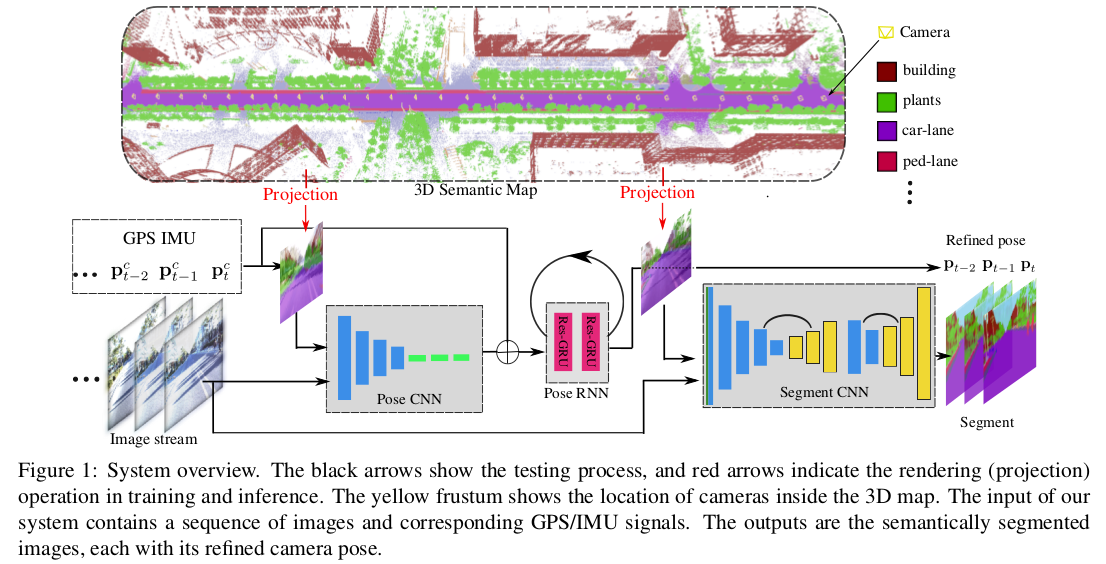
\includegraphics[width=0.95\textwidth]{SemanticSLAM/DeLS1.png}
\caption{DeLS Framwork}
\label{DeLSFramework}
\end{figure}

从图中可以看出,RGB Images 以及 根据GPS/IMU获得的semantic label map被输入到Pose CNN,然后输出的Pose信息输入到Pose RNN来对Pose进一步提高,{\bfseries 这里用RNN来获得前后帧的一致性}!然后在利用新得到的Pose来获取更精确的Semantic Label Map,最后,这个label Map以及RGB图像输入到Segment CNN来进一步提高语义地图的精度。这里标签地图被用于提高语义地图的空间精度以及时间一致性。

网络的训练是基于非常精确地相机姿态以及语义分割,所以可以采用监督学习。

\subsection{Related Work}

\begin{itemize}
\item Camera Pose Estimation

\begin{itemize}
\item PnP

在大的范围内,可能需要提供姿态的先验信息。但对于城市环境中存在大量的Points,这种方法不适用,且不适用于纹理少、结构重复、以及重叠的区域。

\item Deep learned features

PoseNet, LSTM-PoseNet, Bi-Directional LSTM, or Kalman filter LSTM.但实际中由于存在植被等重复性的场景,所以十分有必要加入GPS/IMU等信息来获得鲁棒的定位结果。而在这里,我们采用结合RGB图像与Online Rendered label map的方式来提供更好的结果。

{\bfseries \color{red} 这里问题来了,首先是label map的精度如何?其次,随着时间的变化,label map与实际RGB图像可能完全不同,如季节改变了,这应该如何?}

\end{itemize}

\item Scene Parsing

FCN, Multi-scale context module with dilated convolution, Pooling, CRF, or Spatial RNN with hundreds of layers.这些方法都太耗时了。

一些方法是利用小模型或者模型压缩来加速,但会降低精度。

当输入是Video时,需要考虑时空信息。当前,存在利用光流来帮助label以及semantic在相邻帧之间的传递。借助3D信息以及相机姿态把相邻帧联系起来,可以更好的处理静态背景下的表示。具体的,是使用DeMoN来提高推理效率。

\item Joint 2D-3D for video parsing

CNN-SLAM把传统的3D重建模块替换为深度预测网络,且借助语义分割网络来获取场景语义。同样比较耗时、仅适合静态背景,重建效果也不好。

\end{itemize}

\subsection{Dataset}

\begin{itemize}
\item Data collection

Mobile LIDAR to collect point clouds of the static 3D map. Cameras' resolution: 2018 * 2432.

\item 2D and 3D Labeling

\begin{itemize}
\item Over-segment the point clouds into point clusters based on spatial distances and normal directions, then label each point cluster manually.

\item Prune out the points of static background, label the remaining points of the objects.

\item After 3D-2D projection, only moving object remain unlabeled.

\end{itemize}

\item 使用图形学中的 \textit{Splatting techniques} 来优化未被标签的像素。

\end{itemize}

\subsection{Localizing camera and Scene Parsing}

\subsubsection{Render a label map from a camera pose}

初始的相机的姿态来自于GPS/IMU等传感器。

6-DOF相机姿态:$\mathbf{b} = [\mathbf{q}, \mathbf{t}] \in SE(3)$. 其中$\mathbf{q} \in SO(3)$是四元数表示的旋转,$\mathbf{t} \in \mathbb{R}^3$表示Translation。

在由Point经Spaltting获取其面时,面积大小$s_c$根据Point所属的类别来决定,且与该类别与相机的平均距离的比例有关。

\begin{displaymath}
s_c \propto \frac{1}{|\mathcal{P}_c|}\sum_{x \in \mathcal{P}_c}\min_{\mathbf{t}\in \tau}d(x, t)
\end{displaymath}

其中,$P_c$是属于类别$c$的3D点云,$\tau$是精确地相机姿态。如果面积过大,则会出现Dilated edges,而如果面积过小,则会形成Holes。

\subsubsection{Camera Localization rectification with road prior}

\textbf{CNN-GRU pose Network Architecture}

文中的Pose Network包含一个Pose CNN以及一个Pose GRU-RNN。其中Pose CNN的输入是RGB图像I以及一个标签地图L。输出是一个7维的向量,表示输入图像I与输入标签地图L(由较粗糙的姿态$\mathbf{p}_i^c$得到)之间的位姿关系,从而得到一个在3D Map中更精确的姿态:
$\mathbf{P}_i = \mathbf{p}_i^c + \hat{\mathbf{p}}_i$。

CNN结构借鉴DeMoN,利用打的Kernel Size来获取更大的内容,同时保证运行效率,减少参数量。

由于输入的是图像流,为了保证时间一致性,所以在Pose CNN之后又加上一个多层的GRU网络,且该网络具有Residual Connection的连接结构。结果表明,RNN相比于卡尔曼滤波可以获得更好的运动估计。

\textbf{Pose Loss}

类似于PoseNet的选择,使用Geometric Matching Loss来训练。

\subsubsection{Video Parsing with Pose Guidance}

上一步得到的Pose估计,不是完美的,因为存在light poles存在。由于反光,很多点消失了。此外,由于存在动态物体,这些物体可能在原来的标签地图中不存在,所以这些区域可能发生错误。因此,利用额外的一个Segment CNN来出来这些问题。且利用标签地图来指导分割过程。

\textbf{Segment Network Architecture}

首先基于RGB图像对该网络训练,然后加入标签地图数据进行微调(Fine Tune).具体结构如图\ref{SegmentDeLS}所示。

\begin{figure}[!hbtp]
\centering
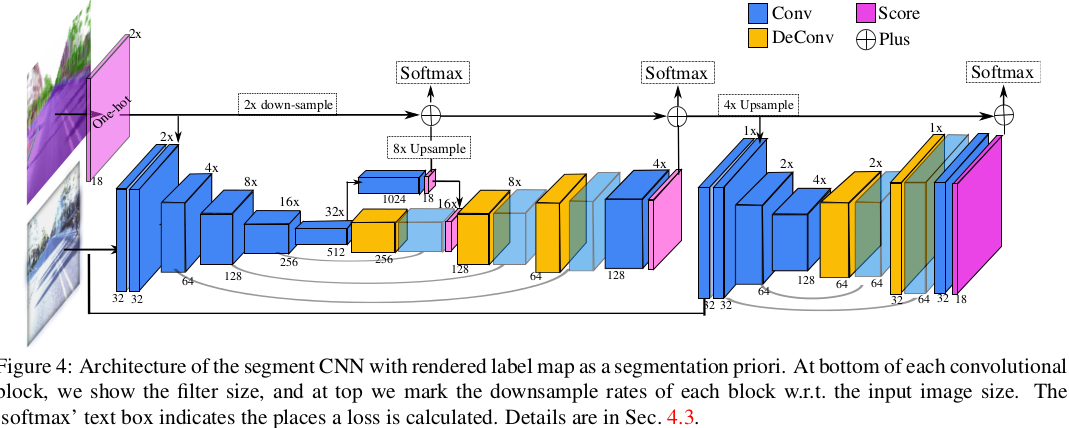
\includegraphics[width=0.95\textwidth]{SemanticSLAM/DeLS2.png}
\caption{Segment Network in DeLS}
\label{SegmentDeLS}
\end{figure}

需要注意的是,当标签地图加入框架时,需要经过编码,即每一个像素经One-hot操作得到一个32维的Feature Representation。然后得到的32维特征加入到RGB图像的第一层卷积输出中,且该层的Kernel数也是32个,从而平衡了两种数据的通道数(Channel Number)。

\subsection{Experiment}

\begin{itemize}
\item Adopt OpenGL to efficiently render a label map with the z-buffer handling. 

\item Implement all the networks by adopting the MXNet platform.

\item 使用RNN可以提高Pose的精度,也可以提高Segment的精度,尤其对于纤细的物体。

\end{itemize}

\subsection{Conclusion}

基于已有的3D语义地图以及视频数据,实现相机的姿态、场景语义任务的实现。算法融合了多种传感器信息。实验表明,相机位姿估计与场景语义两类任务可以相互促进、提高。

\section{PAD-Net: Multi-Task Guided Prediction-and-Distillation Network for Simultaneous Depth and Scene Parsing \cite{Xu2018PADNet}}

\subsection{Abstract}

利用同一个网络,完成深度估计与场景解析两个任务。具体来说,通过神经网络学习一系列的中间辅助任务(Intermediate Auxiliary Tasks),然后基于中间任务的输出,作为多模式数据(Multi-modal  input)输入到下一层网络中,完成最终的深度估计以及场景解析两个任务。

其中,一系列的中间任务包括低层任务和高层任务。低层任务包括:Surface Normal, Contour;高层任务包括:Depth Estimation, Scene Parsing.

\subsection{Analysis}

\subsubsection{Effect of Direct Multi-task Learning}
It can be observed that on NYUD-v2, the Front-end + DE + SP slightly outperforms the Front-end
+ DE, while on Cityscapes, the performance of Front-end + DE + SP is even decreased, which means that using a direct multi-task learning as traditional is probably not an effective means to facilitate each other the performance of different tasks. (DE: Depth Estimation, SP: Scene Parsing)

\subsubsection{Effect of Multi-modal Distillation}
这种Multi-Modal Distillation对结果十分有效。且:
\begin{quote}
By using the attention PAD-Net (Distillation C + SP) guided scheme, the performance of the module C is further improved over the module B.
\end{quote}

\subsubsection{Importance of Intermediate Supervision and Tasks}

测试了选择不同的中间任务类型,如:(Multi-Task Deep Network)MTDN + inp2(depth + semantic map), MTDN+3inp3(depth + semantic + surface normal), MTDN + all(depth + semantic + surface + contour).

其中MTDN + all比MTDN + 0-3都好。

\section{RNN for Learning Dense Depth and Ego-Motion from Video}

参考文献:\cite{Wang2018DenseSLAMNet}

{\color{red}时间:2018年05月19日}

\subsection{Abstract}

现在基于学习的单目深度估计,在Unseen Dataset上泛化较差,可以利用连续两帧之间的特征匹配来解决。本文提出了基于RNN的多目视觉深度估计以及运动估计。结果表明,在远距离上的深度估计,表现很好。本文方法可使用both static and deformable scenes with either constant or inconsistent light conditions.

\subsection{Introduction \& Related Works}

由于CNN只能捕获单帧内部的空间特征,所以即使输入两帧图像,实际效果也比较差。相关的SLAM框架有:

\begin{itemize}
\item ORB-SLAM, DSO: 稀疏SLAM
\item LSD-SLAM: semi-dense SLAM,利用光强来实现跟踪以及构建地图
\item DTAM: dense SLAM
\end{itemize}

上述框架仅适用于静态、光照恒定、足够的camera motion baseline的情景。

进来,CNN可被用于SLAM中的以下部分:
\begin{itemize}
\item Correspondence matching
\item Camera Pose estimation
\item Stereo
\end{itemize}
输出包括:
\begin{itemize}
\item Depth maps
\item point clouds and voxels
\end{itemize}
CNN的优势在于可以适用于纹理较少、表面覆盖、很细等场景下,这些场景对纯使用几何技术来说很难实现。

Newcombe研究表明,多目视觉有助于提高深度估计的精度,而本文作者认为采用相邻几帧可以实现类似的效果。

有作者利用一个非监督生成模型来学习复杂的3D到2D的投影。但这些手段不太适用于Deformable Objects.

\subsection{Network Architecture}

\begin{figure}[!htbp]
\centering
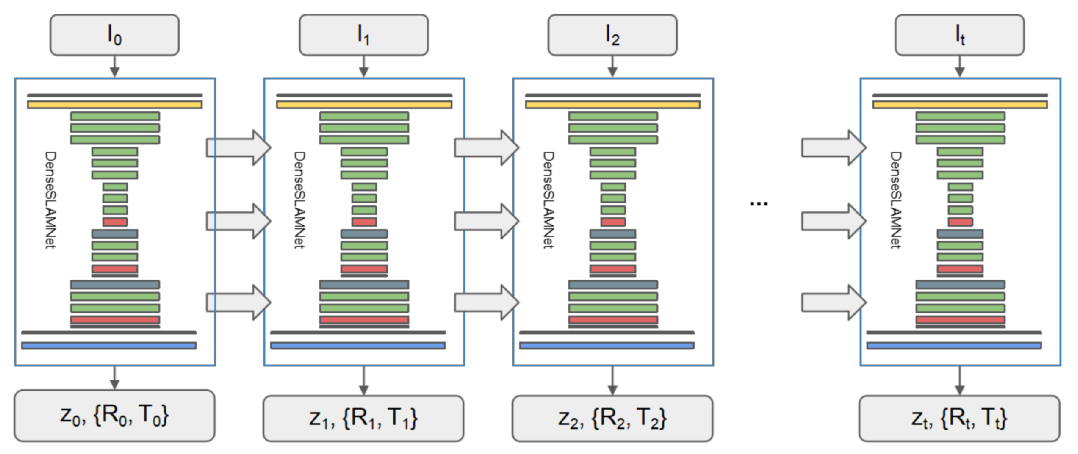
\includegraphics[width=0.95\textwidth]{SemanticSLAM/DenseSLAMNet1.png}
\caption{Dense SLAM框架}
\label{DenseSLAMNet1}
\end{figure}

从图\ref{DenseSLAMNet1}可以看出,它接受当前RGB图像$I_t$以及来自迁移级的隐藏状态$h_{t-1}$。$h_{t-1}$通过LSTM单元进行内部转移。网络的输出是稠密地图$z_t$以及相机的姿态$R_t, T_t$等。有没在每一时刻,只输入一帧图像,且输出该帧对应的深度以及姿态,所以相比于CNN具有更高的灵活性。

具体的每一块的细节结构如下:

\begin{figure}[!htbp]
\centering
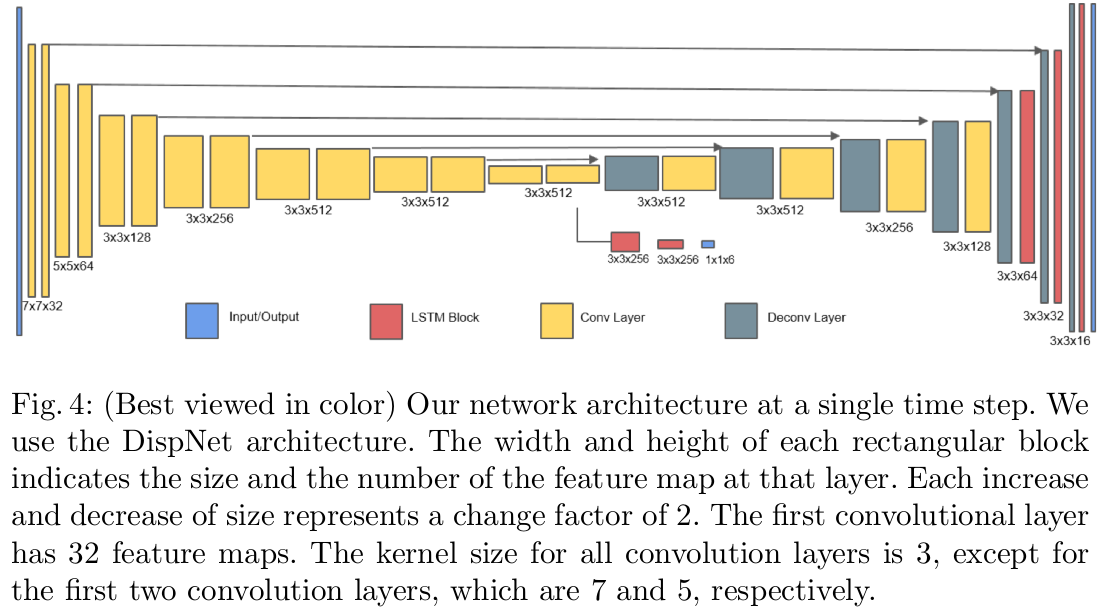
\includegraphics[width=0.95\textwidth]{SemanticSLAM/DenseSLAMNet2.png}
\caption{Dense SLAM中每一级的细节框架}
\label{DenseSLAMNet2}
\end{figure}

网络结构的另一个参数是时间窗口的大小$N$。本文中$N=10$,也就是说,图\ref{DenseSLAMNet2}中的结构被重复十次。

\subsection{Training}

During training, we feed
frames to the network and compute losses from all frames in a temporal window. However, there is no input length constraint at test time.

\subsubsection{Loss Function}

由三部分组成:
\begin{itemize}
\item A Point-wise depth loss

\begin{displaymath}
L_{depth} = \sum_{t}^{N}\sum_{i, j}\left\| \xi_t(i, j) - \hat{\xi}_t(i, j) \right\|_{L1}
\end{displaymath}
其中,$i, j$为索引,$t$为time step.使用$L1-Norm$的原因是,它对噪声更鲁棒。

\item a camera pose loss

Use the Euler angle $R$ 和平移向量$T$。

\begin{displaymath}
\begin{gathered}
L_{rot} = \sum_{t}\left\| r_t - \hat{r}_t \right\|_2 \\
L_{trans} = \sum_{t}\left\| t_t - \hat{t}_t \right\|_2
\end{gathered}
\end{displaymath}

\item a scale-invariant gradient loss

为了保证深度图的Smoothness和Sharpness,所以增加了这个loss。具体如下:
\begin{displaymath}
L_{grad} = \sum_{t}\sum_{h\in\{ 1, 2, 4, 8, 16 \}}\sum_{i, j}\left\| g_{h, t}(i, j) - \hat{g}_{i, j}(i, j)\right\|_2
\end{displaymath}
其中,$h$代表不同的尺度。$g_{h, t}$is a scale-normalized, discretized measurement of the local changes of $\xi_t$。定义如下:
\begin{displaymath}
g_{h, t} = \left( \frac{\xi_t(i+h, j) - \xi_t(i, j)}{|\xi_t(i + h, j) + \xi_t(i, j)|}, \frac{\xi_t(i, j+h) - \xi_t(i, j)}{|\xi_t(i, j+h) + \xi_t(i, j)|}    \right)
\end{displaymath}

$L_{grad}$emphasizes the depth discontinuities, such as occlusion
boundaries and sharp edges, as well as the smoothness in homogeneous regions.
This property encourages the estimated depth map to preserve more details and
reduce noise. Therefore, we put highly weight on this component of the loss. 这一项在所有的Loss中比重较大。

\end{itemize}

最终的Loss由上面几项的和构成:
\begin{displaymath}
L = \alpha * L_{depth} + \beta * L_{pose} + \gamma * L{grad}
\end{displaymath}
其中,$\alpha, \beta, \gamma$是系数,由经验决定。


注意,下面解释的是为什么使用Disparity而不是直接使用深度。
\begin{quote}
{\color{red} \textbf{Caution!} Disparity, the reciprocal of depth (深度的倒数), $\xi = \frac{1}{z}$  as our direct estimation because it can represent points at infinity and account for the localization uncertainty of points at increasing
distance.}
\end{quote}

Different datasets have different camera intrinsic parameters, so we
explicitly crop and resize images to ensure uniform intrinsic parameters. This
step assures that the non-linear mapping between color and depth is consistent
across all training datasets.

\subsection{Experiments}

We evaluate DenseSLAMNet using five error metrics。具体可以参考文章。
\begin{itemize}
\item Sc-inv
\item Abs-rel, Abs-inv
\item RMSE, RMSE-log
\end{itemize}

\subsection{Ablation Studies}

比较了三种不同的网络结构。
\begin{enumerate}
\item CNN-SINGLE, 去掉图\ref{DenseSLAMNet2}中LSTM单元
\item CNN-STACK, 使用与CNN-SINGLE相同的网络,但是输入stack of ten images as input.
\end{enumerate}

实验结果表明,LSTM可有效保留时间域的信息,从而深度预测的更好。

\subsubsection{Conclusions}

引入了LSTM单元。
Our method effectively utilizes the temporal relationships between neighboring
frames through LSTM units, which we show is more effective than simply stack-
ing multiple frames together as input.

比几乎所有的单帧CNN-based 都好。
Our DenseSLAMNet outperformed nearly
all of the state-of-the-art CNN-based, single-frame depth estimation methods on
both indoor and outdoor scenes and showed better generalization ability.


\section[DA-RNN]{DA-RNN: Semantic Mapping with Data Associated Recurrent Neural Networks}

参考文献:\cite{Xiang2017DARNN}

{\color{red} \textbf{评语} 看得出来,RNN在帮助建立相邻帧之间的一致性方面具有很大的优势。}

本文利用可以实现Data Associate的RNN产生Semantic Label。然后作用于KinectFusion,来插入语义信息。

所以本文利用了RNN与KinectFusion来实现语义地图的构建!

\subsection{Related Works}

{\bfseries 本文提出的 DA-RU (Data Associated Recurrent Unit) 可以作为一个单独的模块加入到已有的CNN结构中!}

\subsection{Methods}

需要注意到是,本文采用了DA-RNN与KinectFusion合作的方式来产生最终的Semantic Mapping,而文章采用的则是ORB-SLAM与CNN结合,他们有一些共同的结构,如Data Associate,虽然我现在还不明白这个DA具体得怎么实现!?

\subsection{Experiments}

实验表明,针对不同的实验输入场景,RGB图像和Depth图像可能发挥不同的作用,有一些时候甚至让结果更差,而本文采用Contatenated把来自于RGB和Depth的Feature进行组合起来,在这里,是否可以采取Attention或者\cite{Xu2018PADNet}中采用的Knowledge Distillation的方式进行多模态数据融合呢!?

此外,实验中也发现,有时候RGB图像的Color会影响实验结果,所以,是否可以利用一些其它的不那么Confusing的数据呢,比如Shape等,这也类似于\cite{Xu2018PADNet}中多任务中的Contour类似吧!


\subsection{Conclusion}

\begin{itemize}
\item $\star$将来的可以借助Optical Flow来生成图像帧之间的Data Associate,来代替KinectFusion的作用!
\end{itemize}

\section{SemanticFusion: Dense 3D Semantic Mapping with CNNs}
参考文献:\cite{SemanticFusion2016}

主要框架,用到了ElasticFusion和CNN来产生稠密的Semantic Mapping.

\subsection{Introduction \& Related Works}

本文的算法,利用SLAM来实现2D Frame与3D Map之间的匹配(Corresponding)。通过这种方式,可以实现把CNN的语义预测以概率的方式融合到Dense semantically annotated map.

为什么选择ElasticFusion呢,是因为这种算法是surfel-based surface representation,可以支持每一帧的语义融合。

比较重要的一点是,通过实验说明,引入SLAM甚至可以提高单帧图像的语义分割效果。尤其在存在wide viewpoint variation,可以帮助解决单目2D Semantic中的一些Ambiguations.

之前存在方法使用Dense CRF来获得语义地图。

本文的主要不同是:利用CNN来产生语义分割,然后是在线以 Incremental 的方式生成Semantic Map。即新来一帧就生成一帧的语义地图。

\subsection{Method}

系统由三部分组成:
\begin{itemize}
\item A real-tiem SLAM system ElasticFusion

用于提供帧间的关联、全局一致的地图

\item CNN

产生语义分割

\item Bayesian update scheme

基于SLAM提供的Pose关系、CNN提供的每个像素的Class Probability对Map中的每一个surfel的Class Probability进行更新!

\end{itemize}

此外,作者还尝试了用CRF来利用SLAM提供的Geometry帮助语义分割。

非常粗糙的流程图如下图所示:
\begin{figure}[!hbtp]
\centering
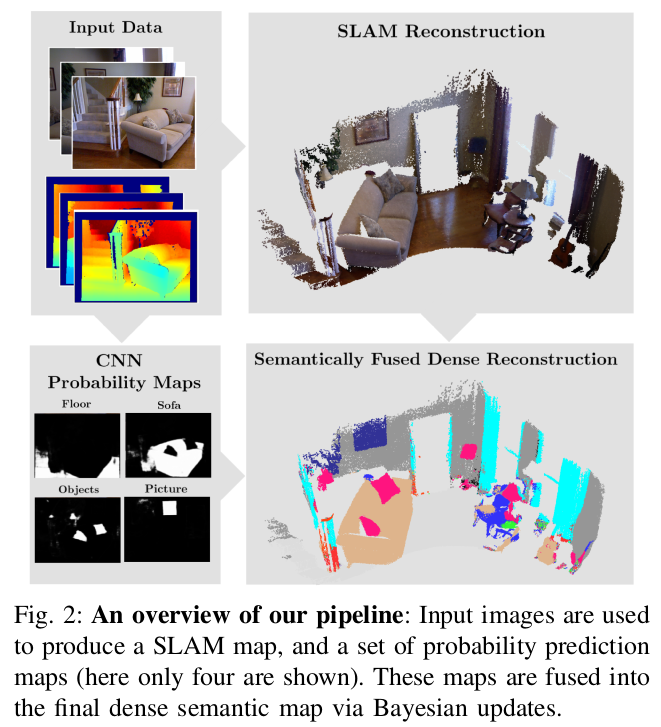
\includegraphics[width=0.75\textwidth]{SemanticSLAM/SemanticFusion0.png}
\caption{粗糙的数据流图}
\label{SemanticFusion0}
\end{figure}

\subsubsection{SLAM Mapping}
就是使用ElasticFusion.

\subsubsection{CNN Architecture}

使用Deconvolutional Semantic Segmentation network,与FCN同年提出的另一个分割网络。

在本实验中,输入由RGB变为RGBD,多了一个Channel.然而,深度相关的训练数据比较少,为了提高利用率,作者利用其它三个输入的光强的平均值对Depth Filter进行初始化。

对输入数据,作者还进行了Scaling, RGB是用Bilinear Interpolation, Depth数据是Nearest enighbour。

\subsubsection{Incremental Semantic Label Fusion}

在生成的地图$\mathcal{M}$中,每一个Surfel(ElasticFusion的结果)不仅代表了Location、Normal等信息,还包含一个类别($\mathcal{L}$)的分布。

输入数据为$\mathbf{I}_k$表示RGB图像与Depth等。

在对每一个Surfel进行类别分布概率更新时,采用的Recursive Bayesian update,这个算法就是Probability Robotics里面最基础的算法,也就是分为Prediction和Correlation两个步骤。

\begin{displaymath}
P(l_i | I_{1, \ldots, k}) = \frac{1}{Z}P(l_i | I_{1, \ldots, k- 1})P(O_{u(s, k)=l_i | I_k})
\end{displaymath}

其中,第一个$P$表示根据过去的信息的预测,在这里也就是已有的$\mathcal{M}$里面的一个surfel的class probability,如果,是一个全新的Surfel,则初始化它为均匀分布,因此这样熵最大;而第二个$P$表示来自CNN输入是$I_k$时输出的class probability,然后对已有地图中的surfel的class probability进行Correlation!

\subsubsection{Map Regularisation}

作者尝试了利用CRF来借助map geometry对预测的Semantic surfel进行Regularise。

在这里,把每一个Surfel当做CRF的一个Node。

这一部分,参考论文吧。

\subsection{Experiments}

本文用到的Semantic分割的方法(CNN + SLAM)与普通的单CNN相比,具有很大的优势。本文的方法是,得到3D的Semantic Map后,重投影到2D图像中。

时间方面,SLAM需要29.3ms,CNN的前向传播用了51.2ms,Bayesian更新用了41.1ms。

\subsection{总结}

未来也还是SLAM与语义分割相互促进吧,达到Semantic SLAM。


\section{Meaningful Maps with Object-Oriented Semantic Mapping}
参考文献:\cite{Meaningful2016}

主要的框架是,利用CNN与ORB-SLAM2来实现Semantic Mapping。{\bfseries 但是都用到了Data Association的操作}!而且本文还是Object-oriented (Instance level) !

\subsection{Introduction \& Related Works}

{\bfseries 重要:}

与已有的方式不同的是,本文的算法不仅分割独立的3D Point,也就是把语义信息投影到3D Point中,而是投影到3D Structure。这样会更有利于场景理解。

已有的SLAM算法得到的结果都是一些几何上的概念,比如:点、面、表面等。另一方面,为了实现与环境交互,必须基于语义地图才行。

\subsubsection{Semantic Mapping}

语义信息与地图构建可能属于两个不同的过程得到。

有一些算法用到了HMM或Dense CRF等。

\subsubsection{Object Detection and Semantic Segmentation}

FCN的缺点是,形成的语义地图一般缺少Notion of independent object instances. 如果只是Pixel-level的labels不能辨别有重叠时物体的身份。

也有一些Instance-level的分割算法,但精度、速度都有待提高。

\subsection{Object Oriented Semantic Mapping}

算法的主要步骤:
\begin{figure}[!hbtp]
\centering
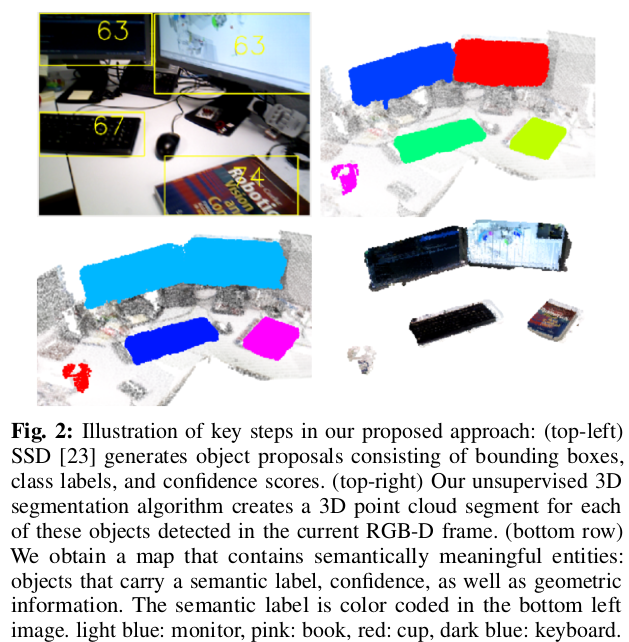
\includegraphics[width=0.75\textwidth]{SemanticSLAM/OrientedMap0.png}
\caption{算法的几个主要步骤}
\label{OrientedMap0}
\end{figure}

算法使用RGB-D作为输入,算法是用ORB-SLAM2提供相机的姿态、地图等。

\subsubsection{Object Detection for Semantic Mapping}

本文使用SSD来完成Object的Location和 Recognition。

\subsubsection{3D Segmentation}

由于需要非常精确的图像分割,所以本文利用Depth图来帮助分割。所以需要对Depth进行分割的算法,本文采用了文章\cite{Felzenszwalb2004}\cite{Pham2016Geometrically}等人的算法。也是涉及到基于图的分割的过程。

\subsubsection{Data Association}

重点。

当完成了把3D Point投影到识别的物体后,数据关联要做的事:判断检测到的物体是否已经在已经构建的地图中存在了呢,如果不存在的话,就需要新增这个物体。

通过一个二阶的流程来实现:

\begin{itemize}
\item 对于每一个检测到的Object,根据点云的欧式距离,来选择一系列的Landmarks(已经检测到并在地图里面已经有的Object)
\item 对Object和Point Cloud of landmark进行最近邻搜索,使用了k-d tree来提高效率,其实这一步也就是判断当前图像检测到的Object与已有的地图中的Landmark(Object)是否相匹配。
\end{itemize}

在第二步中,如果多余50 \% 的Points的都距离小于2cm的话,就说明这个检测到的Object已经存在了。

这个也就是把CNN的分割结果与地图中的Object进行关联起来,并用颜色表示Map中Object的类别。

\subsubsection{Object Model Update}

地图中的目标保存:
\begin{itemize}
\item 与目标相关联的分割的3D点云
\item ORB-SLAM中因子图的各个位姿的索引
\item 有SSD提供的各个目标的置信度
\end{itemize}

\begin{figure}[!hbtp]
\centering
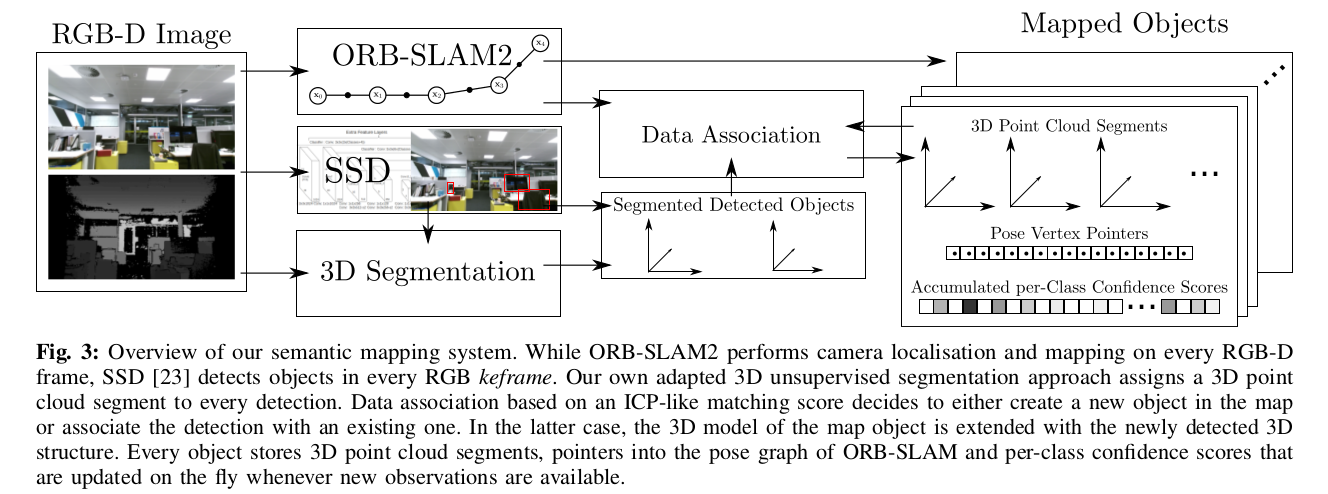
\includegraphics[width=0.95\textwidth]{SemanticSLAM/OrientedMap1.png}
\caption{Semantic Mapping 系统概览}
\label{OrientedMap1}
\end{figure}

上图中可以看出,


{\color{red} \textbf{评语}:在上一篇SematicFusion中,采用的Recursive Bayesian 的更新规则来完成地图更新的!看来,这个是CNN与传统的SLAM框架结合的时候的一个需要解决的问题,那就是如何把新来的物体与已有的地图中的物体相互关联起来,并更新!}

\subsubsection{Map Generation}

通过保存Keyframe中物体的3D poin clouds、每一个物体的3D分割以及执行位姿图中的一个指针。

\subsection{总结}

未来可以的发展方向:
\begin{itemize}
\item 语义Landmark如何提高SLAM的精度,从而实现Semantic SLAM
\item 把稀疏的语义地图改进为稠密地图
\end{itemize}

\section[LiteFlowNet]{LiteFlowNet: A Lightweight Convolutional Neural Nework for Optical Flow Estimation}

参考文献:\cite{Hui2018LiteFlowNet}, CVPR 2018

\subsection{背景知识}

FlowNet2是基于CNN进行光流估计的SOTA算法(?), 需要160M的参数量。LiteFlowNet实现了30倍的轻量化,并且比FlowNet2块1.36倍。

主要的贡献:
\begin{itemize}
\item 在每一层金字塔(Pyramid Level)预测光溜更高效的轻量级联网络。通过早前矫正(Early Correction)提高了精度,同时无缝支持网络中的描述子匹配。
\item 提出了一个新型的光流正则化层,可以改善野值点、光流边界模糊等问题,是基于特征驱动的区域卷积实现
\item 网络结构可以高效提取Pyramidal Feature以及Feature Warping,而不是像FlowNet2中的Image Warping。
\end{itemize}

FlowNet2通过级联FlowNet,来不断调优光流场, by contributing on the flow increment between the first image and the warped second imaeg?

后来,SPyNet通过在每一Pyramid level采用Imae Warping实现了只有1.2M大小的网络,但精度只有FlowNet大小,而达不到FlowNet2的水平。

{\bfseries Image Warping: 图像扭转,是一种数字图像处理过程,在任何图像中所描述的任何形状都会产生显著有损。扭曲可用于矫正图像有损,同时可用于某种创意目的。纯粹的图像扭曲意味着点到点的映射,而不改变其颜色。}

提高FlowNet2以及SPyNet的两种准则(Principles):

\begin{itemize}
\item Pyramid feature extraction

Consists of an encoder and a decoder. Encoder把输入的图像对分别映射到多尺度高维特征空间中;Decoder以Coarse-to-fine的框架估计光流场。这比FlowNet2采用U-Net更轻量化。相比于SPyNet,我们的模型把特征提取与光流估计两个过程分离,可以更好的处理精度与复杂度之间的矛盾。

\item Feature Warping

FlowNet2与SPyNet将输入图像对中的第二幅图像基于先前估计的光流进行Warp,然后使用Warped的第二幅图像与第一幅图像的特征图谱Refine估计的光流。

所以这个过程中,首先把第二幅图像进行Warp,然后提取Warp图像的特征,这个过程十分繁琐。所以,本文提出直接对Feature Map进行warp。保证模型更精确以及高效。

\end{itemize}

更详细的细节一定要看原文\cite{Hui2018LiteFlowNet}。

此外,除了上面两个主要改进的 Principle, 作者还提出第三个比较重要的改进措施,那就是 Flow Regularization.

\begin{itemize}
\item Flow Regularization

级联的光流估计类似于能量最小化方法中的保真度(Data Fidelity)的作用。 为了消除边界的模糊以及野值点,Regularize flow Field的常用Cues:
\begin{itemize}
\item Local flow consistency
\item Co-occurrence between flow boundaries
\item Co-occurrence between intensity edges
\end{itemize}

对应的代表方法包括:
\begin{itemize}
\item Anisotropic image-driven
\item image- and flow-driven
\item Complementary regularizations
\end{itemize}

在本文中,提出的是Feature-driven local convolution layer at each pyramid level. 该方法对Flow-以及Image-敏感。

{\color{red} \textbf{评语}:看起来,一个是提高精度,一个是提高效率,这是两个最终的目的。提高精度可以通过设计网络结构以及增加其它考虑来实现;提高效率的一个重要表现是降低模型的参数数量,提高运算速度。不过,本文虽然参数数量减少了30倍,但速度却只提高了1.36倍,这里面的原因是什么?}

\end{itemize}

\subsection{Related Works}

\subsubsection{Variational Methods}

Address illumination changes by combining the brightness and gradient constancy assumptions.

DeepFlow, propose to correlate multi-scale patches and incorporate this as the matching term in functional.

PatchMatch Filter, EpicFlow.

本文提出的网络结构,是受Variational methods中的Data Fidelity以及正则化启发。

\subsubsection{Machine Learning Methods}

PCA-Flow. 这些参数化模型可以通过CNN高效的实现。

\subsubsection{CNN-based Methods}

FlowNet, 使用能量最小化作为后处理步骤,来降低在光流边界的平滑效应。不能端到端训练?

FlowNet2, 通过FlowNet的级联实现。虽然提高了精度,但模型更大,计算更复杂。

SPyNet,受Spatial Pyramid启发,模型更紧凑,但效果远不如FlowNet2。

InterpoNet, 借助第三方系数光流但需要off-the-shelf的边缘检测。

DeepFlow, 使用Correlation而不是真正意义的CNN,参数不能训练。

\subsubsection{Establish Point Correspondence}

Establishing point correspondence, 一种方式是Match Image Patches

CNN-Feature Matching, 首先被Zagoruyko等人提出(Learning to compare image patches via CNN, 2015 CVPR)。

MRF-based, G$\ddot{u}$ney等人提出利用Feature Representation以及利用MRF来估计光流。

Bailer使用多尺度Feature,然后以类似于Flow Fields的方式进行特征匹配。

Fischer和Ilg等人为了提高计算效率,仅在稀疏空间维度进行特征匹配。

本文中,We reduce the computational burden of feature matching by using a short-ranged matching of warped CNN features at sampled positions and a sub-pixel refinement at every pyramid level.

类似于Spatial Transformer, 本文利用 f-warp layer来区分不同个Channel.本文的决策网络是一个更普用的Warping Network,可以用来Warp高层次的CNN Features,而不仅仅是对Image进行Warpping.


\subsection{LiteFlowNet}

整体结构如下:
\begin{figure}[!hbtp]
\centering
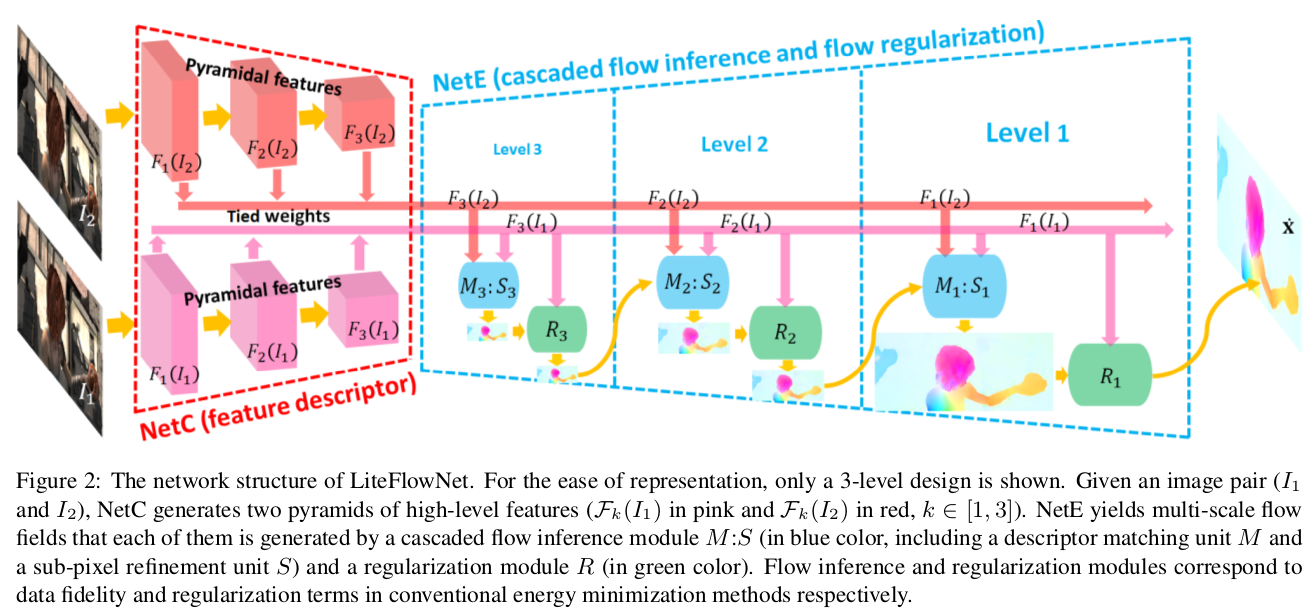
\includegraphics[width=0.95\textwidth]{SemanticSLAM/LiteFlowNet0.png}
\caption{LiteFlowNet结构框图}
\label{LiteFlowNet0}
\end{figure}

\subsubsection{Pyramid Feature Extraction}

进行stride-$s$的卷积操作,得到的Feature Map表示为:$\mathcal{F}_k(I_i)$,即第$i$个图像的第$k$层Feature Map。简化写成 $\mathcal{F}_i$。

\subsubsection{Feature Warping (f-warp)}

假设\.x为预测的光流,则Feature Warping是指:
\begin{displaymath}
\tilde{\mathcal{F}}_2(x) \triangleq \mathcal{F}_2(x + \dot{x}) \sim \mathcal{F}_1(x) 
\end{displaymath}

注意,Warping是作用于$\mathcal{F}$上的,而不是输入图像上的。

为了使上述过程可以支持end-to-end训练,这里采用Bilinear Interpolation进行插值的技术实现Warping。Bilinear Interpolation是支持后向传播训练的!修改后Warping实现公式如下:
\begin{displaymath}
\tilde{\mathcal{F}} = \sum_{x_s^i \in N(x_s)} \mathcal{F}(x_s^i)(1-|x_s - x_s^i|)(1 - |y_s - y_s^i|)
\end{displaymath}

其中,$x_s = x + \dot{x} = (x_s, y_s)^T$是输入的源Feature Map中的坐标。$x$denotes the target coordinates of the regular grid in the interpolated feature map $\mathcal{F}$,$N(x)$代表the four pixel neighbors of $x_s$.

自己的理解:首先$x$是插值后 的图像索引,而$x_s = x + \dot{x}$是插值前Feature Map中对应Object Feature的$x$索引处的索引。$x_s^i$是在$x_s$周围的四个紧邻像素。也就是个Bilinear Interpolated.

\subsubsection{Cascaded Flow Interface}

{\color{red} \textbf{评语}:这一块看的比较吃力。为什么会吃力?因为新的概念么?那么作者为什么提出这么麻烦的概念呢?实际效果又怎么样呢?}

通过计算高层特征向量的Correlation来实现输入图像的点对应。

\begin{displaymath}
c(x, d) = \mathcal{F}_1(x) \cdot \mathcal{F}_2(x + d) / N
\end{displaymath}
这个公式跟FlowNet中的计算方式区别不大。只不过这里的$N$是指Feature的长度。

\begin{figure}[!hbtp]
\centering
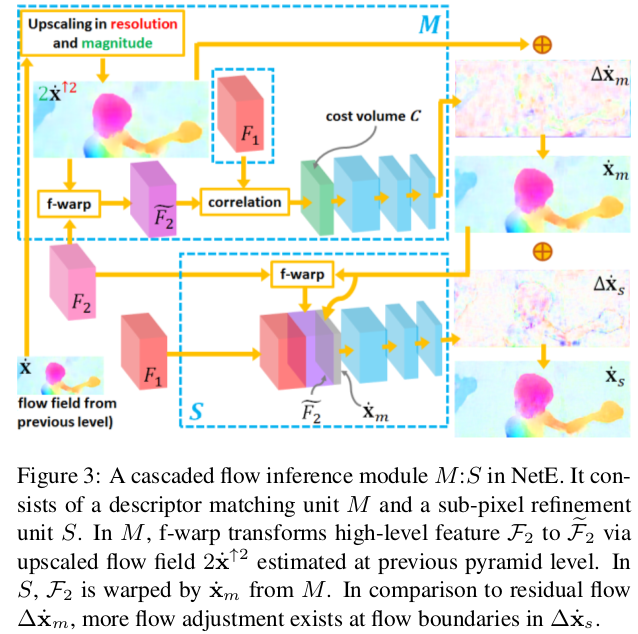
\includegraphics[width=0.75\textwidth]{SemanticSLAM/LiteFlowNet1.png}
\caption{在NetE中的级联光流推理模块,M:S}
\label{LiteFlowNet1}
\end{figure}

\textbf{M Module}$\;$  在Descirptor Matching unit M, Residual flow $\varDelta \dot{x}_m$. A complete flow field $\dot{x}_m$ is computed as follows, 这句话没懂

\begin{displaymath}
\dot{x}_m = \underbrace{M(C(\mathcal{F}_1, \tilde{\mathcal{F}}_2; d))}_{\varDelta \dot{x}_m} + s\dot{x}^{\uparrow s}
\end{displaymath}

其中,$\dot{x}$是上一层的最开始的光流估计!

\textbf{S Module}$\;$ 
为了进一步提高flow estimate  $\dot{x}_m$ 的精度,即达到亚像素级别。作者引入了Second flow inference。 这可以防止错误光流的放大并传到下一级。Sub-pixel refinement unit $S$,会产生一个更准确的光流场,这通过最小化$\mathcal{F}_1$和 $\tilde{\mathcal{F}}_2$之间的距离来实现。

\begin{displaymath}
\dot{x}_s = \underbrace{S(C(\mathcal{F}_1, \tilde{\mathcal{F}}_2, \dot{x}_m))}_{\varDelta \dot{x}_s} + \dot{x}_m
\end{displaymath}

{\bfseries 所以总的来说} M模块是为了计算$\varDelta \dot{x}_m$, 而$S$模块是为了计算$\varDelta \dot{x}_s$。对最开始$\dot{x}$估计的光流进行两次的Refinement.

\subsubsection{Flow Regularization}

这一部分主要消除光流边界的模糊、存在的artifacts等。提出用 feature-driven local convolution (f-lcon)

假设Feature Map (F)的尺寸为:$M * N * c$,定义f-lcon的滤波器为$\textbf{G}={g}$

对于输入为$\dot{x}_s$, Flow Regularization值的是:
\begin{displaymath}
\dot{x}_r = R(\dot{x}_s; G)
\end{displaymath}
输出的是正则化后的光流估计$\dot{x}_r$

下面的关键是如何生成这个用于正则化的卷积核。为此,作者定义了一个feature-driven的距离度量$\mathcal{D}$,总的来说,该度量由一个CNN unit $R_D$来计算:
\begin{displaymath}
\mathcal{D} = R_D(\mathcal{F}_1, \dot{x}_s, O)
\end{displaymath}

基于这个度量,可以计算得到卷积核:
\begin{displaymath}
g(x, y, c) = \frac{\exp(-\mathcal{D}(x, y, c)^2)}{\sum_{(x_i, y_i)\in N(x, y)}\exp(-\mathcal{D}(x_i, y_i, c)^2)}
\end{displaymath}

其中$N(x)$表示一个$\omega * \omega$的近邻。

\subsection{Ablation Study}

算法的结果是优于 FlowNet2, SPyNet等。

\subsubsection{Feature Warping}

没有Warping, 光流更Vague.通过计算residual flow (M:S两个模块的功能)可以提高估计效果。

M: Matching

S: Sub-pixel refinement

R: Regularization units in NetE

\subsubsection{Descriptor Matching}

\subsubsection{Sub-Pixel Refinement}

The flow field generated from
WMS is more crisp and contains more fine details than
that generated from WM with sub-pixel refinement dis-
abled.

更小的flow artifacts.

\subsection{Regularization}

In comparison WMS with regularization
disabled to ALL, undesired artifacts exist in homogeneous
regions

Flow bleeding and
vague flow boundaries are observed.

表明, Feature-driven local convolution对于光滑光流场、保持crisp flow boundaries非常重要!

\subsection{Conclusion}

Pyramidal feature extrac-
tion and feature warping (f-warp) help us to break the de
facto rule of accurate flow network requiring large model
size. To address large-displacement and detail-preserving
flows, LiteFlowNet exploits short-range matching to gener-
ate pixel-level flow field and further improves the estimate
to sub-pixel accuracy in the cascaded flow inference. To
result crisp flow boundaries, LiteFlowNet regularizes flow
field through feature-driven local convolution (f-lcon). With
its lightweight, accurate, and fast flow computation, we ex-
pect that LiteFlowNet can be deployed to many applications
such as motion segmentation, action recognition, SLAM,
3D reconstruction and more.


\section{小结}

2018.05.23小结

在生成Semantic Map的时候,看样子现在的趋势,是利用RNN保证时间一致性;利用多模态数据提高精度,但如何融合多模态数据的Feature有待研究,现有的有一些是直接Concatenate、Knowledge Distillation、Attnetion(?)等机制。


\section{ExFuse: Enhancing Feature Fusion for Semantic Segmentation}

参考文献:\href{https://zhuanlan.zhihu.com/p/37177073}{ExFuse简介-知乎}

\subsection{要解决的问题}

在语义分割领域中,经常需要融合多层的Feature。然而,底层的Feature含有的语义信息较少,但分辨率较高,噪声也比较少,这是由于卷积层比较浅;而高层的Feature语义信息多,但空间分辨率很小。

所以本文就提出了:1)增加底层特征的语义;2) 在高层中增加空间信息

\subsection{Method}

使用了ResNet、GCN(Global Convolution Net)的思想。

\begin{figure}[!hbtp]
\centering
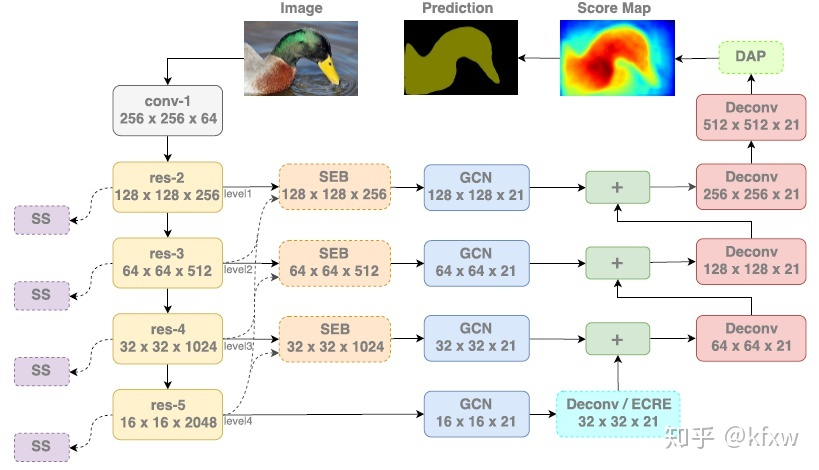
\includegraphics[width=0.95\textwidth]{SemanticSLAM/ExFusion0.jpg}
\caption{ExFusion的实现框图}
\label{ExFusion0}
\end{figure}

其中,SS, SEB, ECRE, DAP是文章作者提出的算法。

\subsubsection{在底层中加入更多的语义信息}
具体是三个方面的改进:
\begin{itemize}
\item Layer Rearrengement

 ResNeXt网络结构中,各级的网络包含的残差单元个数为{3,4,23,3}。为了提高底层特征的语义性,一个想法便是让低层的两级网络拥有的层数更多。因此作者将残差单元个数重排为{8,8,9,8},并重新在ImageNet上预训练模型。重排后网络的分类性能没有明显变化,但是分割模型可以提高约0.8个点(mean intersection over union)的性能。

\item Semantic Supervision(SS)

深度语义监督其实在其他的一些工作里(如GoogLeNet,边缘检测的HED等等)已经使用到了。这里的使用方法基本上没有太大变化,能够带来大约1个点的提升。

\item Semantic Embedding branch(SEB)

\begin{figure}[!hbtp]
\centering
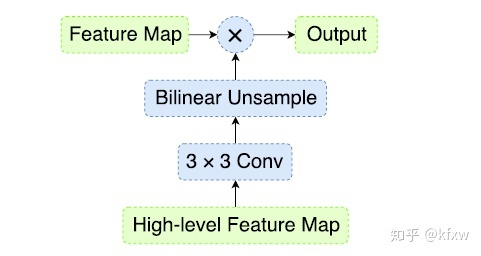
\includegraphics[width=0.65\textwidth]{SemanticSLAM/ExFusion1.jpg}
\caption{语义嵌入分支的结构图}
\label{ExFusion1}
\end{figure}

 其做法是将高层特征上采样后,与低层特征逐像素相乘,用在GCN之前。该部分能带来大约0.7个点的提升。

\end{itemize}

\subsubsection{在高层中加入更多的空间信息}

用两种方法来把更多的空间信息融入到高层特征中:
\begin{itemize}
\item 通道分辨率嵌入(Explicit Channel resolution embedding, ECRE)

其思路是在上采样支路中使用[2,3,4]工作中都使用到的子像素上采样模块(sub-pixel upsample)。作者的出发点并不是前人工作中强调的如速度快、消除反卷积的棋盘效应等等,而是通过这个结构能够让和空间信息相关的监督信息回传到各个通道中,从而让不同通道包含不同空间信息。该模块和原有的反卷积一起使用才能显示出更好的性能。同单独使用反卷积相比,性能可以提高约0.6个点。

\item 稠密邻域预测(Densely adjacent prediction, DAP)

DAP模块只使用在输出预测结果的时候。其想法也是通过扩展通道数来增加空间信息。举一个例子来描述其功能,假设DAP的作用区域为3x3,输出结果的通道数为21,则扩展后的输出通道数为21x3x3。每3x3个通道融合成一个通道。如在最终结果中,第5通道(共21通道)的(12,13)坐标上的像素,是通过DAP之前的第5+0通道(11,12)、5+1通道的(11,13)、5+2通道的(11,14)、5+3通道的(12,12)、5+4通道的(12,13)、5+5通道的(12,14)…平均得到的。DAP能带来约0.6个点的提升。

\end{itemize}

\section{Multi-View Deep Learning for Consistent Semantic Mapping with RGB-D Cameras}

{\color{red} 时间:2018.05.24}

主要的贡献是:以自监督的方式预测多视角一致的语义分割,在与关键帧的语义地图融合时,更加一致。

\subsection{Introduction \& Related Works}
现阶段,RGB-D数据,Appearance以及Shape Modalities对于语义分割都会有帮助,可以结合起来。但结合多视觉信息的做法,还没有人尝试。

那么如何把多视觉Frames与SLAM结合起来呢,作者的做法是,根据SLAM提供的Pose,其中一个帧为目标帧,目标帧存在Ground Truth 标签数据,然后,同一时刻其它视角的Frame可以通过SLAM计算得到的位姿被Warp到目标帧中。这样,网络可以学习视角不变的特性,且不需要额外的标签数据。其它视角的输出被Warp到目标帧(Reference)中,然后融合,融合过程是以概率的形式完成的。

\subsubsection{Image based Semantic Segmentation}

有一些是单独利用RGB输入,有一些输入是RGB-D数据。

前者,主要的思想有FCN、Encoder-decoder结构通过可学习的Unpooling, Deconvlution等完成语义分割。

后者,有一些基于encoder-decoder的可以融合RGB数据与Depth数据,也可以吧Depth数据转换成HHA, 其它的还有Mulit-scale Refinement, dilated Convolutions以及Residual units,此外还有LSTM来融合RGB与Depth数据,可生成更平滑的结果。最后,还有一些用到了CRF的算法。

{\color{red} \textbf{评语}:如果输入数据是RGB-D数据的话,那么就不用像\cite{Xu2018PADNet}那样需要额外的单独预测Depth的网络结构了,而直接使用Attention或Knowledge Distillation等机制处理Depth与RGB数据不就可以了么!?}

\subsubsection{Semantic SLAM}

SLAM++可以实现Object Instance level的跟踪、地图构建等。

其它的一些算法包括概率的形式融合语义信息。还有是处理点云的算法。


\subsubsection{Multi-View Semantic Segmentation}

CNN用于多目3D的语义分割研究很少。

存在用3D CNN来处理系数的Octree数据结构,得到对voxel的语义分割。

有算法提出使用视频中的Superpixel和Optical Flow来融合视频中的多目视觉的语义信息。

跟本文相近的一个算法是利用多目来实现Shape Recognition中。


\subsection{CNN Architecture For Semantic Segmentation}

本文在FuseNet上的改进是,加入了Multi-scale的Loss Function Minimization。

\begin{figure}[!hbtp]
\centering
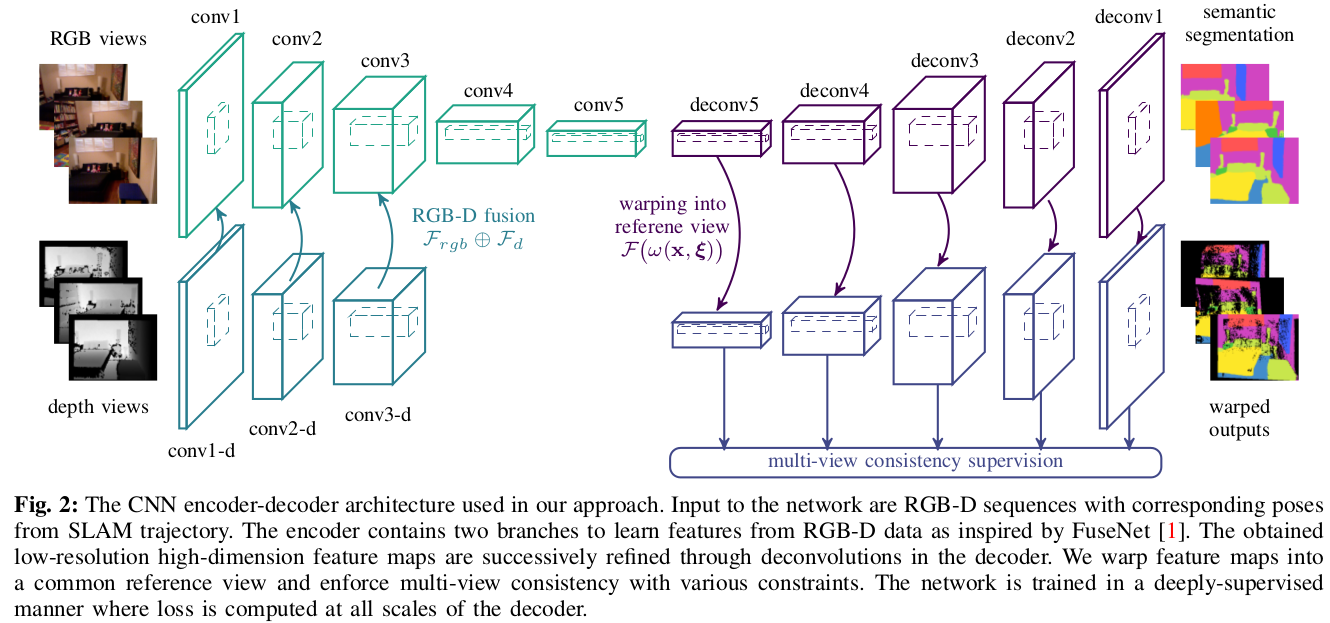
\includegraphics[width=0.95\textwidth]{SemanticSLAM/MultiView0.png}
\caption{基于Encoder-Decoder CNN的语义分割示意图}
\label{MultiView0}
\end{figure}

需要注意到有一下几点:
\begin{itemize}
\item 使用Unpooling、Deconvolution等实现Decoder
\item 注意,RGB与Depth经过两个分离的分支提取特征,然后在多个尺度(Multi-scale!)进行融合!
\item 使用KL散度作为Loss Function :

\begin{displaymath}
L(\mathcal{W}) = - \frac{1}{N} \sum_{i}^{N}\sum_{j}^{K}\lfloor j = l_{gt} \rceil \log p_j (x_i, \mathcal{W} | \mathcal{I})
\end{displaymath}

\item 使用Deeply Supervised Learning method计算all Upsample Scales,注意,Gound Truth使用\textbf{Stochastic Pooling}这种正则化技术生成各个尺度下对应的Gound Truth
\end{itemize}

\subsection{Multi-View Consistent Learning and Prediction}

本文的主要贡献是,Explore the use of temporal multi-view consistency within RGB-D sequences for CNN training and prediction. 这是通过把多帧数据Warp到一个Common Reference View来实现。

\subsubsection{Multi-view Data Associate Through Warping}

为了保证时间一致性,引入了Warping Layers。

该Layer的操作原理是:
\begin{displaymath}
X^{\omega} = w(x, \xi) = \pi (T(\xi)\pi^{-1}(x, Z_i(x)))
\end{displaymath}
其中,$\omega$为Warping function, $T(\xi)$为SLAM得到的位姿$\xi$下的单应变换;$\pi$实现3D坐标与图像坐标之间的转换。$Z_i(x)$为图像$x$处的深度信息。

\subsubsection{Consistency Through Warp Augmentation}

把KeyframeWarp到Neighboring Frames。

\subsubsection{Consistency Through Bayesian Fusion}

\begin{align}
p(y|z^i) & = \frac{p(z_i|y, z^{i-1})p(y | z^{i-1})}{z_i|z^{i - 1}} \notag \\
         & = \beta_i p(z_i | y, z^{i-1}) p(y | z^{i-1}) \notag
\end{align}

其中,$z^i$为到达第$i$帧的所有Measurements。

上式也就是Recursive Bayesive Update.

\subsubsection{Consistency Through Multi-View Max-Pooling}

Bayesian Fusion是在Probability域内进行的,而这里作者还尝试了直接在Feature域内进行Fuse。

使用Multi-View max-pooling对Warp 的 Feature Map进行处理。

\subsection{Experiments}

使用NYUDv2数据集、DVO-SLAM框架。

使用Cubic Interpolation来对RGB图像进行降采样,利用Nearest-neighbor Interpolation来对Depth和Labelling数据进行降采样

使用SGD Moment训练,动量为0.9,同时有0.0005的Weight Decay。Learning Rate 被设置为0.001然后每30K次迭代就Decay by a factor of 0.9。

使用IOU来判断Segment的效果。

\subsection{总结}

We base our CNN design on FuseNet,a recently proposed CNN architecture in an encoder-decoder scheme for semantic segmentation of RGB-D images.

All multi-view consistency training approaches outperform single-view trained baselines. They are key to boosting segmentation performance when fusing network predictions from multiple view points during  testing.

In future work, we want to further investigate integration of our approach in a semantic SLAM system, for example, through coupling of pose tracking and SLAM with our semantic predictions.

所以,作者的意思是说现在还没有达到Semantic SLAM的水平,而实现的也就是只有Semantic Segmentation吗!?SLAM只是提供了必要的位姿估计,来帮助相邻帧之间的Warping?

\section[MaskFusion]{MaskFusion: Real-Time Recognition, Tracking, and Reconstruction of Multiple Moving Objects}

MaskFusion,看样子挺厉害的样子。

A real-time, object-aware, semantic And dynamic RGB-D SLAM.({\color{red} 为什么这几篇基于RGB-D数据的算法这么多呢!?所以,要发文章的话,可以选面向不同输入数据的一种方法!比如,双目的文章我还没有看到,虽然上篇是关于Multi-View的语义分割,但不涉及SLAM啊。看样子生成语义地图的结果应该会挺炫的。})

可以实现更有优势的Instance-level的Semantic Segmentation。利用VR应用来表明MaskFusion的独特优势:Instance-aware, Semantic and Dynamic。

\subsection{背景及相关工作}

把SLAM应用到AR(Augemented Reality)时,还有两个问题解决的不太理想:
\begin{itemize}
\item 现在的SLAM系统均假设环境是静态的,会主动忽略Moving Objects
\item 现在的SLAM系统得到的均是一些几何的地图,缺少语义信息。有一些尝试,如SLAM++, CNN-SLAM
\end{itemize}

本文提出的MaskFusion算法可以解决这两个问题,首先,可以从Object-level理解环境,在准确分割运动目标的同时,可以识别、检测、跟踪以及重建目标。

分割算法由两部分组成:
\begin{itemize}
\item Mask RCNN

提供多达80类的目标识别等。

\item A geometry-based segmentation algorithm

利用Depth以及Surface Normal等信息向Mask RCNN提供更精确的目标边缘分割。

\end{itemize}

上述算法的结果输入到本文的Dynamic SLAM框架中。

使用Instance-aware semantic segmentation比使用pixel-level semantic segmentation更好。{\bfseries 目标Mask更精确,并且可以把不同的object instance分配到同一object category}。

本文的作者又提到了现在SLAM所面临的另一个大问题:Dynamic的问题。作者提到,本文提出的算法在两个方面具有优势:
\begin{itemize}
\item 传统的Semantic SLAM尝试

相比于这些算法,本文的算法可以解决Dynamic Scene的问题。

\item 解决Dynamic SLAM的尝试

本文提出的算法具有Object-level Semantic的能力。

\end{itemize}

{\color{red} \textbf{评语}:所以总的来说,作者就是与那些Semantic Mapping的方法比Dynamic Scene的处理能力,与那些Dynamic Scene SLAM的方法比Semantic能力,在或者就是比速度。确实,前面的作者都只关注Static Scene, 现在看来,实际的SLAM中还需要解决Dynamic Scene(Moving Objects存在)的问题。}

\subsubsection{Dense RGB-D SLAM}

KinectFusion证明使用Truncated Signed Distance Function(TSDF)可以表示室内地图构建,此外,其它的工作也证明使用合适的数据结构也可以完成室外环境的地图构建。

Surfels: Surface Elements, 在Computer Graph中应用比较早。

Surfel类似于Point Cloud,不同的是,Surfel不仅包含Location信息,还包含Radius和Normal等,此外,不像Point Cloud下在切换Mapping与Tracking之间时的Overhead.且是高效存储的。

\subsubsection{Scene Segmentation \& Semantic Scene Segmentation}

单纯的Scene Segmentation可以提供精确的目标边界,但缺乏Semantic Information.

Semantic Scene Segmentation作者只提到了基于MRFs的方法。

\subsubsection{Semantic SLAM \& Dynamic SLAM}

Semantic SLAM中提到了CNN-SLAM, Semantic Fusion

{\color{red} \textbf{评语}: 但作者的意思是这些算法没有考虑Object instance level的语义分割,而只考虑点云层面的分割,如果真是这样的话,那么不就没多少意义了,当然对人来说可能很清楚,但对机器而言,必须考虑Object Instance level.好像,这两个算法中确实就是这样。}

存在两种方法可以处理Dynamic SLAM的问题,而不把Moving Object当做Outlier来处理:
\begin{itemize}
\item Deformable world is assumed and as-rigid-as-possible registration is performed
\item Object instances are identified and potentially tracked rigidly
\end{itemize}

上面两种方法都涉及要么Template- 要么是 descriptor-based methods

\subsection{System Design}

\subsubsection{System Overview}

\begin{figure}[!hbtp]
\centering
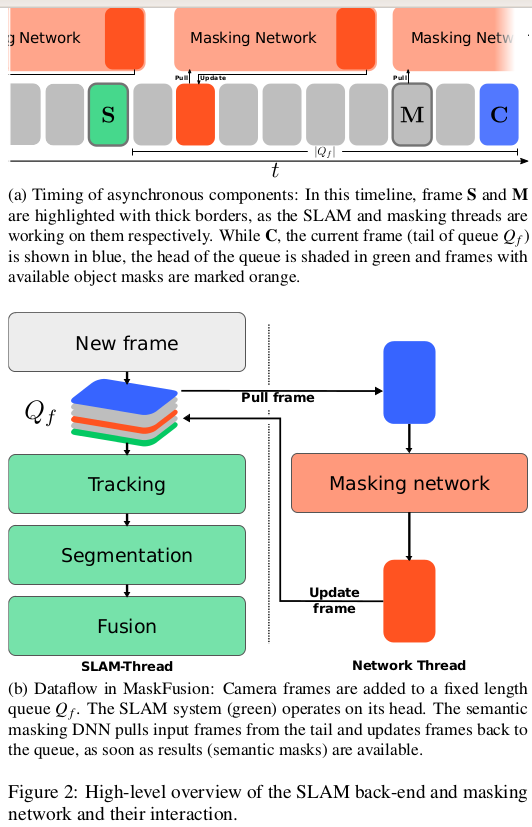
\includegraphics[width=0.85\textwidth]{SemanticSLAM/MaskFusion0.png}
\caption{Overview of MaskFusion}
\label{MaskFusion0}
\end{figure}

每新来一帧数据,整个算法包括以下几个流程:
\begin{enumerate}
\item Tracking

每一个Object的6 DoF通过最小化一个能量函数来确定,这个能量函数由两部分组成:几何的ICP Error, Photometric cost?。此外,作者仅对那些Non-static Model进行Track。最后,作者比较了两种确定Object是否运动的方法:
\begin{itemize}
\item Based on Motioin Incosistency
\item Treating objects which are being touched by a person as dynamic
\end{itemize}

\item Segmentation

使用了Mask RCNN和一个基于Depth Discontinuities and surface normals 的分割算法。前者有两个缺点:物体边界不精确、运行不实时。后者可以弥补这两个缺点, 但可能会Oversegment objects。

\item Fusion

就是把Object的几何结构与labels结合起来。

\end{enumerate}

\subsubsection{Multi-Object SLAM}

本文采用ElasticFusion类似的3D Model.其中,Model用Surfel来表示,Surfel具体包含以下内容:
$\mathcal{M}_m^s \in \{ \mathbf{p}\in\mathbb{R}^3, \mathbf{n}\in\mathbb{R}^3,\mathbf{c}\in\mathbb{N}^3,\mathbf{w}\in\mathbb{R},\mathbf{r}\in\mathbb{R}, \mathbf{t}\in\mathbb{R}^2  \}, \forall s < |\mathcal{M}_m|$, 分别表示:Position, normal, color, weiht, radius, and two timestamps.此外,系统还包含每一个目标的Label $l_m =m \forall m \in 0 \ldots N$, $N$是场景中包含的Object的数量。

这一步SLAM主要解决的问题是,对Ojbect的Pose的跟踪,由于输入时RGB-D数据,且像前面说的那样,作者的目标函数包含两个部分:
\begin{itemize}
\item Geometry Error

\begin{displaymath}
E_m^{icp} = \sum_{i}\left( (v^i - exp(\xi_m)v_t^i)\cdot n^i  \right)^2
\end{displaymath}

其中,$\xi_m$表示待求解的用6DoF李代数表示的相机位姿。$v^i, v_i^t$分别表示第$i$个vertex in surfels, 以及领一帧图像在这上面的投影。

\item Photoconsistency residuals

把输入的RGB图像转化成灰度图:$r, g, b \rightarrow 0.114r + 0.299g + 0.587b$, 然后这一部分的误差$E_m^{rgb}$参考论文。

\end{itemize}

总的目标函数就是两者之和:
\begin{displaymath}
E_m = \min_{\xi_m} \left( E_m^{icp} + E_m^{rgb} \right) 
\end{displaymath}

在完成Pose的跟踪后,然后跟下面的分割结果进行Associate。

这一步并不是每一帧都这样处理。

\subsubsection{Segmentation}

本部分主要包括三个小模块:
\begin{itemize}
\item Semantic Instance Segmentation

这部分就是Mask RCNN来做。

\item Geometric Segmentation

这一部分借鉴了别人的做法,在Depth图中引入两个概念:$\Phi_d$ Depth Discontinuity term, Concavity term $\Phi_c$, 然后如果$\Phi_d + \Phi_c > \tau$那么该点就是位于一个边缘上,是分割点。$\tau$是一个阈值。$\Phi_c, \Phi_d$在邻域上计算。

更多细节,看论文。

这一步是每一帧都会这样处理。

\item 如何把上面两个分割结果整合到一起,然后在与Map整合到一起

第一步与第二步并不是完全一致的,如果match了,才会整合到一起,平时用第二步比较多。

\begin{itemize}
\item Mapping geometric segmentation to Mask

根据Maximal Overlap进行匹配。

\item Mapping Mask to Model

\end{itemize}
\end{itemize}

\subsection{Evaluation}

使用了ATE、RPE、RMSE等评价指标。

\subsection{总结}

总的来说,本文算是一个大杂烩,亮点不是很明显啊,虽然在开始的地方,作者强调了几个本文解决的重要问题,但实际上,文中并没有看到清晰的对这些问题的解决。可能是我没看明白。

不过,在Geometry Segment这一块,作者借鉴了另一个工作,这与其它算法有点不同,其它的都是基于CNN的实现?输入是Depth数据,而作者这里没有用到CNN网络,而是通过一种邻域阈值的方法实现的。

另外一点就是,Tracking的时候,可能通过引入上面提到的两种不同的误差项就可以实现多目标跟踪吧,结果存疑,然后公式写的还那么非主流。

总体而言,并不好,前面的讨论倒是挺开拓视野的。


\section{小结 2}

现在看来语义SLAM主要的研究点:
\begin{itemize}
\item 输入数据:

单目、多目、RGB-D数据等,如果是单目等,可能就需要单独的SLAM框架来提供相机的Pose以及Depth, 如果提供了Depth可以考虑用CNN进行处理两种模式的数据。

\item 实时性

\item Semantic SLAM

现在要实现Object Instance-level,不能再是Point-level了,不然对于系统而言,可做的事情减少很多,因为只有认识Object Instance才能更好的交互,反而如果只有一堆Point的分类,对于机器系统用处不大吧,可能。

\item Dynamic SLAM

如何处理好Moving Object的问题。

\item 输出数据:

稠密还是稀疏?

\end{itemize}


\section[CNN-SLAM]{CNN-SLAM:}

{\color{red} 时间:2018.05.25}




\section{图像语义分割之FCN和CRF}

参考文章:\href{https://zhuanlan.zhihu.com/p/22308032}{图像分割2017.7-知乎}

知乎上专栏总结的一个总体分割框架:
\begin{figure}[!hbtp]
\centering
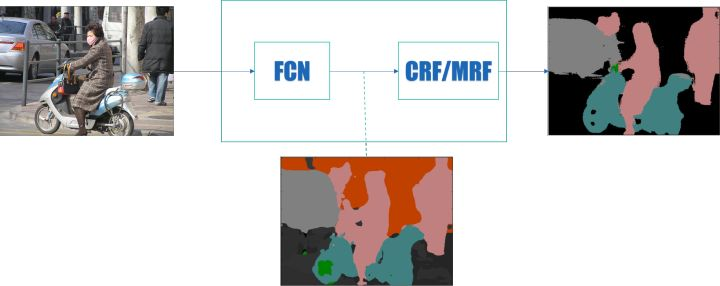
\includegraphics[width=0.85\textwidth]{SemanticSLAM/ImageSegmentFrame0.jpg}
\caption{图像分割的算法框架}
\label{ImageSegmentFrame0}
\end{figure}

前端使用FCN进行特征粗提取,后端使用CRF/MRF优化前端的输出,最后得到分割图。 

\subsection{前端FCN}

\subsubsection{FCN}

主要用到了三种技术:
\begin{enumerate}
\item 卷积化

卷积化即是将普通的分类网络,比如VGG16,ResNet50/101等网络丢弃全连接层,换上对应的卷积层即可。

\item 上采样

此处的上采样即是反卷积(Deconvolution)。当然关于这个名字不同框架不同,Caffe和Kera里叫Deconvolution,而tensorflow里叫conv\_transpose。CS231n这门课中说,叫conv\_transpose更为合适。

众所诸知,普通的池化(为什么这儿是普通的池化请看后文)会缩小图片的尺寸,比如VGG16 五次池化后图片被缩小了32倍。为了得到和原图等大的分割图,我们需要上采样/反卷积。

反卷积和卷积类似,都是相乘相加的运算。只不过后者是多对一,前者是一对多。而反卷积的前向和后向传播,只用颠倒卷积的前后向传播即可。所以无论优化还是后向传播算法都是没有问题。具体的原理,需要参考DLTips一章。

\item 跳跃结构

这个结构的作用就在于优化结果,因为如果将全卷积之后的结果直接上采样得到的结果是很粗糙的,所以作者将不同池化层的结果进行上采样之后来优化输出。

\end{enumerate}

\subsubsection{SegNet/DecovNet}

这两种结构可以直接参考原文,因为就只有结构的图示,没有详细解释。

\subsection{DeepLab}

首先这里我们将指出一个第一个结构FCN的粗糙之处:为了保证之后输出的尺寸不至于太小,FCN的作者在第一层直接对原图加了100的padding,可想而知,这会引入噪声。

而怎样才能保证输出的尺寸不会太小而又不会产生加100 padding这样的做法呢?可能有人会说减少池化层不就行了,这样理论上是可以的,但是这样直接就改变了原先可用的结构了,而且最重要的一点是就不能用以前的结构参数进行fine-tune了。所以,Deeplab这里使用了一个非常优雅的做法:将pooling的stride改为1,再加上 1 padding。这样池化后的图片尺寸并未减小,并且依然保留了池化整合特征的特性。 

但是,事情还没完。因为池化层变了,后面的卷积的感受野也对应的改变了,这样也不能进行fine-tune了。所以,Deeplab提出了一种新的卷积,带孔的卷积:Atrous Convolution.即图\ref{DeepLabAtrousConvolution0}所示。

\begin{figure}[!hbtp]
\centering
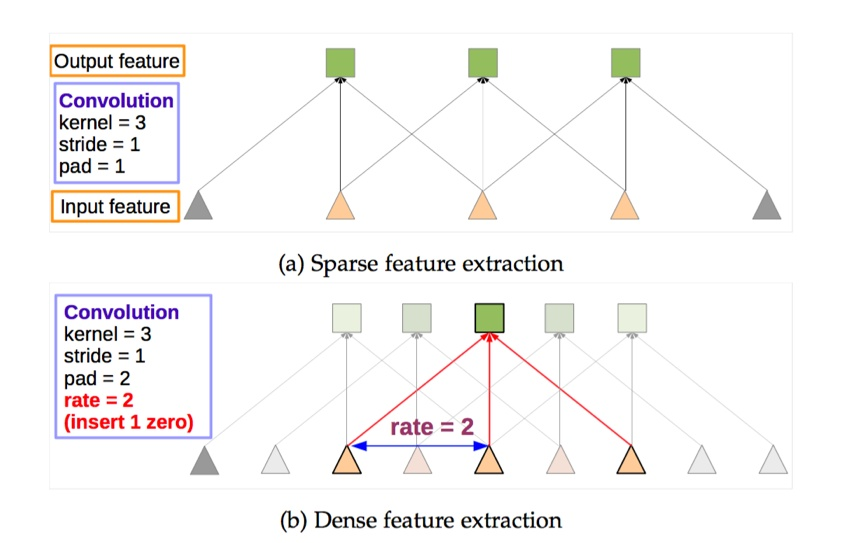
\includegraphics[width=0.75\textwidth]{SemanticSLAM/DeepLabAtrousConvolution0.jpg}
\caption{Atrous Convolution 示意图}
\label{DeepLabAtrousConvolution0}
\end{figure}

具体的感受野变化:

\begin{figure}[!hbtp]
\centering
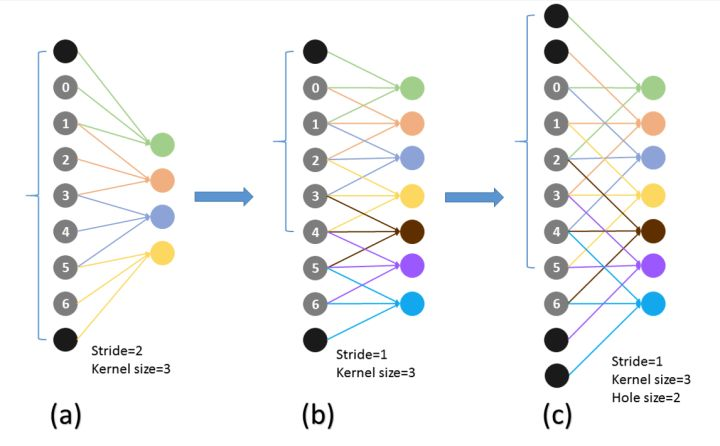
\includegraphics[width=0.85\textwidth]{SemanticSLAM/DeepLabAtrousConvolution1.jpg}
\caption{Atrous Convolution中的感受野变化 示意图}
\label{DeepLabAtrousConvolution1}
\end{figure}

图\ref{DeepLabAtrousConvolution1}中,a为普通的池化的结果,b为“优雅”池化的结果。我们设想在a上进行卷积核尺寸为3的普通卷积,则对应的感受野大小为7.而在b上进行同样的操作,对应的感受野变为了5(与a中颜色相同的输出所对应的输入只有0, 1, 2, 3 ,4。所以感受野变为5了。).感受野减小了。但是如果使用hole为1的Atrous Convolution则感受野依然为7.判断感受野的过程是,在输出数量一致的情况下(即和a中的输出的4种颜色相同的输出),所覆盖的输入的个数。

所以,Atrous Convolution能够保证这样的池化后的感受野不变,从而可以fine tune,同时也能保证输出的结果更加精细。

其实就是Dialted Convolution的思想。

\subsection{后端优化CRF/MRF}

\subsubsection{全连接CRF, DenseCRF}

对于每个像素$i$具有类别标签$x_i$还有对应的观测值$y_i$,这样每个像素点作为节点,像素与像素间的关系作为边,即构成了一个条件随机场。而且我们通过观测变量$y_i$来推测像素$i$对应的类别标签$x_i$。也就是说,这里的观察值$y_i$为对应第$i$位置的像素。

二元势函数就是描述像素点与像素点之间的关系,鼓励相似像素分配相同的标签,而相差较大的像素分配不同标签,而这个“距离”的定义与颜色值和实际相对距离有关。所以这样CRF能够使图片尽量在边界处分割。

在这里,势函数的输入来自FCN的输出。

而全连接条件随机场的不同就在于,二元势函数描述的是每一个像素与其他\textbf{所有}像素的关系,所以叫“全连接”。 

\subsubsection{CRFasRNN}

最开始使用DenseCRF是直接加在FCN的输出后面,可想这样是比较粗糙的。而且在深度学习中,我们都追求end-to-end的系统,所以CRFasRNN这篇文章将DenseCRF真正结合进了FCN中。

这篇文章也使用了平均场近似的方法,因为分解的每一步都是一些相乘相加的计算,和普通的加减(具体公式还是看论文吧),所以可以方便的把每一步描述成一层类似卷积的计算。这样即可结合进神经网络中,并且前后向传播也不存在问题。

当然,这里作者还将它进行了迭代,不同次数的迭代得到的结果优化程度也不同(一般取10以内的迭代次数),所以文章才说是as RNN。

\subsubsection{马尔科夫随机场, MRF}

没看懂,但还是把原文贴过来了。论文是:Deep Parsing Network

算了,还是去看论文吧,虽然我还没看。

\subsubsection{高斯条件随机场, G-CRF}

\subsection{小结}

2017.07.06

\begin{itemize}
\item FCN更像一种技巧。随着基本网络(如VGG, ResNet)性能的提升而不断进步。
\item 深度学习+概率图模型(PGM)是一种趋势。其实DL说白了就是进行特征提取,而PGM能够从数学理论很好的解释事物本质间的联系。 
\item 概率图模型的网络化。因为PGM通常不太方便加入DL的模型中,将PGM网络化后能够是PGM参数自学习,同时构成end-to-end的系统。

\end{itemize}

\section{Learning Deconvolution Network for Semantic}
参考文献:\href{https://zhuanlan.zhihu.com/p/26291607}{Learning Deconvolution Network for Semantic 1-知乎}

\href{https://zhuanlan.zhihu.com/p/27580384}{Learning Deconvoluton Network for Semantic 2-知乎}

背景:
FCN具有以下限制:
\begin{itemize}
\item 固定尺寸的感受野。对于对于大尺度目标,只能获得该目标的局部信息,该目标的一部分将被错误分类;对于小尺度目标,很容易被忽略或当成背景处理

\item 目标的细节结构容易丢失,边缘信息不够好。FCNs得到的label map过于粗糙,而用于上采样的反卷积操作过于简单

\end{itemize}

本文的主要贡献:
\begin{itemize}
\item 提出了可学习的反卷积网络, 并将其首次应用于语义分割
\item 分割结果是Instance-wise的分割,所以摆脱了原来FCNs中的尺度问题,这也是对应FCNs中的第一个问题
\item 在Pascal Voc12测试集上得到一个很好的效果,与FCN8s模型融合,得到当时最好的准确率
\end{itemize}

\begin{figure}[!hbtp]
\centering
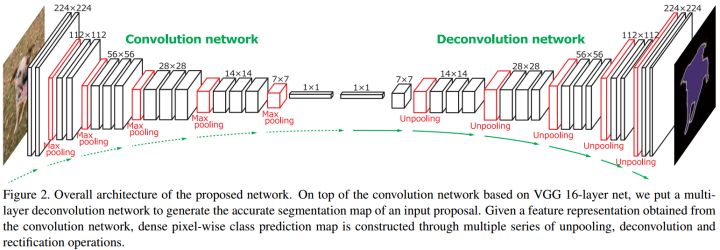
\includegraphics[width=0.95\textwidth]{SemanticSLAM/LearnDeconv0.jpg}
\caption{论文提出的神经网络结构}
\label{LearnDeconv0}
\end{figure}

反卷积网络主要由unpooling层、deconv层、relu层、BN层组成。

\subsubsection{Instance-wise Segmentation}

每张图片被裁剪为很多子图片,每张子图片包含一个目标实例。每张子图片作为输入,得到分割结果,再把这些分割结果聚合起来,得到整张图片的分割图。

\section[ReSeg 2015]{ReSeg: A RNN-based Model for Semantic Segmentation}

参考文献:\cite{ReSeg2015}

基于ReNet实现,每一层ReNet基于四个RNN实现,这四个RNN分别对应水平、垂直方向的双向信息。此外, ReNet is stacked在CNN之上,可以利用Generic local features。在ReNet之后,是提高分辨率的网络。

\subsection{背景 \& 相关工作}

普通的CNN会极大降低分辨率。FCN类的方法不能很好的利用local和global contextual dependencies, 而这些已被证明对分割具有较大帮助。因此,这些模型也经常利用CRF等作为后端处理,来locally smooth the model predictions, 但对于long-range contextual dependencies还是没有被很好的研究过。

而RNN可已被用于retrieve global spatial dependencies, 但是计算量较大。In this paper, we aim at the efficient application of Recurrent Neural Networks RNN to retrieve contextual information from images.

ReNet的每一层可以通过先水平扫描,然后垂直扫描来提高获取global information的能力。

在相关工作中,RNN可以实现分析长距离像素之间的关系,因此被用于语义分割中。ReNet具有很高的并行性,因为每一行之间的计算是相互独立的,每一列的处理也是独立并可以并行计算。

\subsection{Model Description}

首先,输入图像被送入在ImageNet上预训练好的VGG16网络。

然后,输出的Feature Maps被送进ReNet层,该结构可以sweep over输入的feature maps。

最后,多个Upsampling layer被用于把最后的Feature map的分辨率恢复到输入图像的分辨率的大小,接着,用Softmax进行分类。

使用GRU来很好的平衡存储量与计算能力的开销。

\subsubsection{Recurrent layer}

结构如图\ref{ReSeg0}所示。

\begin{figure}[!hbtp]
\centering
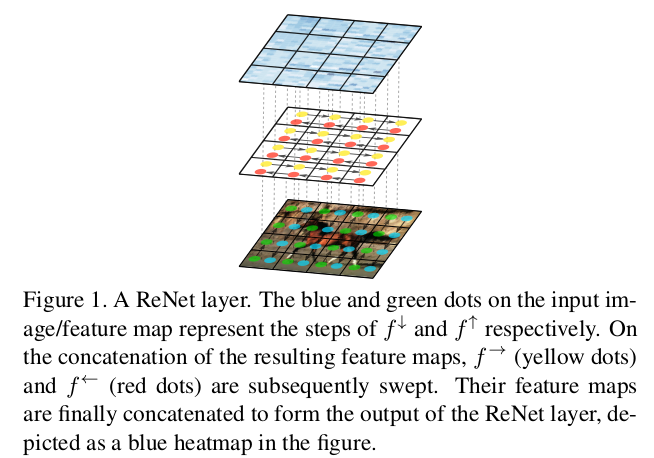
\includegraphics[width=0.75\textwidth]{SemanticSLAM/ReSeg0.png}
\caption{ReNet layer结构}
\label{ReSeg0}
\end{figure}

其中, $f^{\downarrow}$与$f^{\uparrow}$分别表示垂直方向两个方向的RNN, 具有U Recurrent unit结构?



\subsubsection{Upsampling layer}

作者说有三种提高分辨率的方法:
\begin{itemize}
\item Fully Connected layers

这种方法不适合,没有考虑输入的拓扑结构

\item Full convolutions

这种方法需要大的Kernel与Stride size等

\item Transposed Convolutions

这个方法好,既Memory efficient又Computation Efficient。

\end{itemize}

Transposed Convolution, 又被称为 Fractionally strided convolutions.下面是比较有意思的解释:
\begin{quote}
Convolution is based
on the observation that direct convolutions can be expressed
as a dot product between the flattened input and a sparse
matrix, whose non-zero elements are elements of the convolutional kernel. The equivalence with the convolution is
granted by the connectivity pattern defined by the matrix.

Transposed convolutions apply the transpose (转置) of this
transformation matrix to the input, resulting in an operation whose input and output shapes are inverted with respect to the original direct convolution.
\end{quote}

上一段的引用,详情可以从参考第八章中关于Deconvolution的说明,是一致的,且还有例子!

关于Deconvolution的更多说明可以参考:A guide to convolution arithmetic for deep learning.

\subsection{实验结果}

数据集:

Weizmann Horse, Oxford Flowers 17, CamVid Dataset.

使用IoU。

一个重要的现象:当数据集是Highly imbalanced, 分割效果会极大的变差, 因为此时网络会最大化那些经常出现的类别的分数, 而忽略不经常出现的类别?。为了解决这个问题,作者在Corss-entropy loss中加入了一个新的项,来bias the prediction towards the low-occurrence classes.

具体的就是:\textbf{Median Frequency Balancing}。

which re-weights the class predictions by the ratio between the median of the frequencies of the classes
(computed on the training set) and the frequency of each class. This increases the score of the low frequency classes (see Table 4) at the price of a more noisy segmentation mask, as the probability of the underrepresented classes is overestimated and can lead to an increase in misclassified pixels in the output segmentation mask.

\subsection{总结}

The proposed architecture shows state-of-the-art performances on
CamVid, a widely used dataset for urban scene semantic
segmentation, as well as on the much smaller Oxford Flowers dataset. We also report state-of-the-art performances on the Weizmann Horses.

\section[U-Net]{U-Net: CNN for Biomedical Image Segmentation}

参考文献:\cite{U-Net2015}

本文的一大贡献:证明通过更好的使用数据增广来提高现有训练数据的利用率。

另一大贡献,是提出一种结构,该结构由Contracting和Expanding两个部分组成,这一点与FlowNet类似啊。	

结果表明,仅需要非常少的图像数据就可以实现不错的效果。

\subsection{Network Architecture}

本文提出的网络结构实在FCN基础上进行的改进。

网络结构如图\ref{U-Net0}所示。

\begin{figure}[!hbtp]
\centering
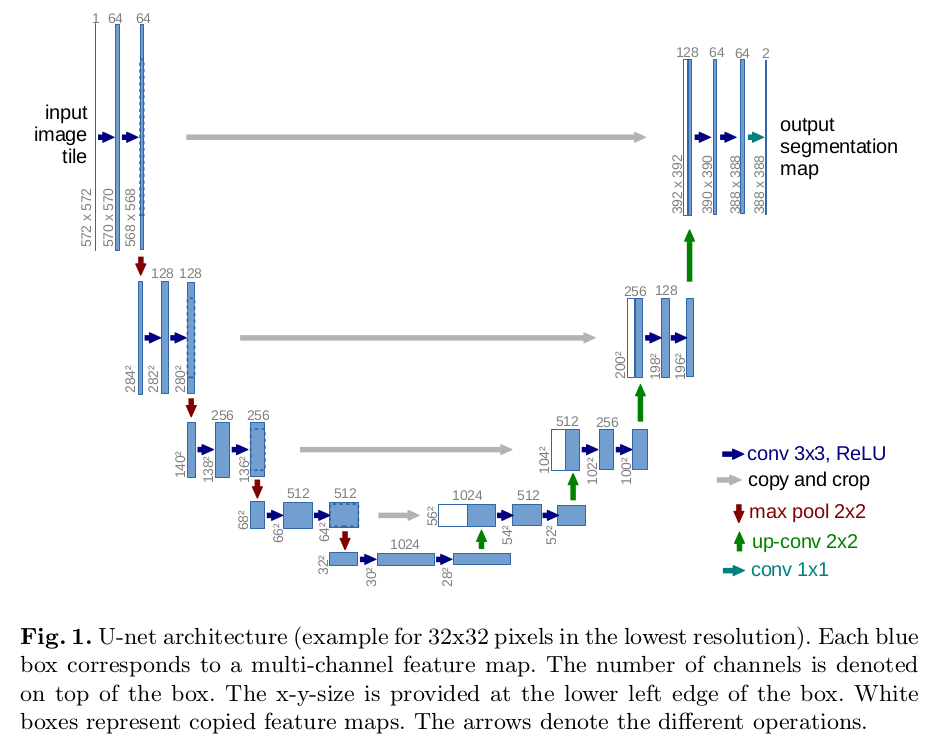
\includegraphics[width=0.8\textwidth]{SemanticSLAM/U-Net0.png}
\caption{U-Net结构示意图}
\label{U-Net0}
\end{figure}

与FCN不同的是,U-Net把结构分成Contracting与Expanding两个Path, Contracting部分与普通的卷及网络相同。It consists of the repeated
application of two 3x3 convolutions (unpadded convolutions), each followed by
a rectified linear unit (ReLU) and a 2x2 max pooling operation with stride 2
for downsampling. At each downsampling step we double the number of feature
channels.

而Expanding部分与FCN中不同的在于,其Feature Channel特别多,与Contracting中基本对称的一样多。每一层包含一个'Up-Convolution', 同时把Feature Channel数量减半。

在最后一层,一个1 * 1 的Convolution被用于把64-Component feature vector映射到目标的number of classes。

Contracting部分的Feature Map与Expanding Path部分的Feature Map会进行\textbf{Concatenation}, 这一点与FCN也不同。U-Net是在Channel维度进行拼接,而FCN是逐点相加!参考文章:\href{https://zhuanlan.zhihu.com/p/31428783}{FCN/U-Net结构解析-知乎}, 这一点属于特征融合步骤的不同!

在训练过程中,用到了Cross Entropy作为目标函数,同时进行数据增广:Shift, Rotation, Deformation, Gray value variantions.

貌似Random elastic deformation对于训练少量Label的数据来说非常重要。We generate smooth
deformations using random displacement vectors on a coarse 3 by 3 grid. The
displacements are sampled from a Gaussian distribution with 10 pixels standard
deviation. Per-pixel displacements are then computed using bicubic interpola-
tion. Drop-out layers at the end of the contracting path perform further implicit
data augmentation.


\subsection{Conclusion}

Thanks to data augmentation with elastic deformations (弹性变形), it only needs very few annotated images and has a very reasonable training time of only 10 hours on a NVidia Titan GPU (6 GB).

\subsection{补充}
\begin{itemize}
\item U-Net中的'Up-Convolution'是什么意思?

知乎上有文章说,就是用的Deconv来实现的。

\item 在最后的几层,如何把Feature map映射成语义分割图像呢?这在FCN\cite{Fcn2014}中也是之前被忽略的问题。

其实在最后的输出层也是一个Feature map, 它的Channel数量就是目标类别的数量,比如,在在Pacal中类别数为21(包括Background), 所以输出的最后的Feature Map具有21个Channel,这个可以参考FCN论文中的图1.另外,在图\ref{U-Net0}中也可以看出,最后的输出通道数为2,即每一类别代表一个channel,然后利用SoftMax进行在Channel维度上进行计算,得到对应像素的类别结果。这一步一般通过一个1*1的Convolution来实现。这一点也可以参考下面FCN论文中的原话:
\begin{quote}
	We append a 1 × 1 convolution with chan-
	nel dimension 21 to predict scores for each of the PAS-
	CAL classes (including background) at each of the coarse
	output locations, followed by a deconvolution layer to bi-
	linearly upsample the coarse outputs to pixel-dense outputs
	as described in Section 3.3.
\end{quote}

这么说来,原来Fully Convolution是这个意思,即相当于在原来Fully Connect的层在空间维度上进行扩充扩充,最终的结果是,现在每一个像素位置都对应于一个原来Fully Connect的维度的Vector!
\end{itemize}

总结一下, CNN图像分割基本上套路是:
\begin{itemize}
\item 下采样 + 上采样: Convolution + Deconvolution /Resize
\item 多尺度特征特征融合:如Concatenate或者逐点相加
\item 获得像素级的Segment Map, 一般通过n * 1*1 Convolution得到,其中$n$为类别数目。
\end{itemize}

\section{Semantic Visual Localization}

参考文献: \cite{SemanticVisualLocalization2017}
妹的,21页。

看样子,本文的主要主要关注点在于建立:Robust visual localization under a wide range of viewing condition.

本文提出利用使用联合\textbf{3D Geometry }和 \textbf{Semantic understanding of the world} 来帮助解决这个问题。

提出的算法, 利用一个新提出的生成模型来完成descriptor learning, 该过程trained on semantic scene completion as an auxiliary task.

最终,得到的3D descriptors可以很鲁棒,可以借助高层的3D geometric 以及 语义信息来处理丢失Observe的情况。

看样子,本文算法比较新颖,效果也很好,一个比较大的优势是采用了生成模型,而不是常用的判别模型。

\subsection{背景 \& 相关工作}

其实这篇文章主要的关注点是Localization, 也就是新的传感器数据来了后,怎么更加准确的与地图中的信息进行匹配,难点在于:The main challenge in this setting is successful data association between the query and the database.

为什么难呢,因为实际的场景是经常变化的,所以很容易就匹配错误了。一般的做法是基于描述子之间的匹配来定位,且通过提高描述子的质量来提高定位的质量。这种方法还是不好,比如尺度性不好、需要大量的匹配计算等。

本文提出了一种高效的描述子学习算法, 是基于生成模型而不是判别模型实现的。本文证明了,通过引入Semantics提供了strong cues 对于场景补全。而且不需要人为操作,就可以泛化到其它数据集以及其它传感器类型,并且都不需要重新训练!(生成模型这么强么还是本文的算法很强?)

生成的是3D 描述子。需要解决的一个重要问题是物体遮挡的场景(Occlusion),本文提出的算法通过借助Semantic Completion这一辅助任务来实现遮挡问题的解决。

本文的算法本质上还是提高Descriptor的生成质量以及匹配速度,在Euclidean space内完成。效果来看,可以在不同光照、季节变换等场景下实现定位。

优点没看明白。在相关工作中,作者分析了大量的已有的算法的缺点,我记得的主要的缺点就是:生成的Descriptor不鲁棒或不满足要求、匹配过程复杂、对多变场景处理不好等等。

\subsection{Semantic Visual Localization}

从上文可以看出,作者的主要贡献是:在Eculidean生成包含语义的3D Descriptor, 可以满足场景的多变、快速匹配、很高的精确度等需求。 

模型的输入数据:1) A set of color images with associated depth maps, 2) database image, including their respective camera poses.

算法过程:
\begin{enumerate}
\item 对于Database的一个子set, 预先生成其语义地图:$M_D$
\item 对于Query的一张或多张图像生成其语义地图$M_Q$
\item 建立$M_D$与$M_Q$之间的匹配,得到相机的位姿估计$\mathcal{P}_Q$
\end{enumerate}

上述算法过程,得到的结果,作者认为就可以实现对Extreme viewpoint和光照的鲁棒了。Semantic information is
comparatively invariant to these types of transformations through higher-level scene abstraction.

额,貌似走着不是对输入的RGB图像进行提取Descriptor, 而是对Semantic Maps提取Descriptors!这也行么?

按照上面三个步骤,具体内容如下:
\begin{itemize}
\item Semantic Segmentation and Fusion

首先生成所有输入图像的Dense pixelwise semantic segmentation, 然后把这些分割结果融合到\textbf{3D} Voxel maps $M_D$与$M_Q$。 

任务的目的是计算把Query 和 database map之间最佳匹配的位姿$P \in SE(3)$。

下面给出如何在缺少观察的情况下,通过对场景的语义理解来建立鲁棒的Semantic Maps。

\item Generative Descriptor Learning

又强调了一次:Semantic scene understanding is key to learning such an invariant function.

传统方案中, 有两种方式提高这种Invariant, 一种是学习更好的Matching function, 一种是学一种更好的Embedding。前者效果较好,但计算量很大,因为要比较每一对的Descriptor, 后者计算量小,本文的算法只需要每一个Descriptor计算一次就好。

具体使用一个Encoder来对Scene Semantics 和 Geometry进行编码。为了可以推理出没观察到的部分,算法还涉及一个Semantic scene completion的辅助任务, 同时推理Scenen Semantic 和 Geometry。整个结构如图\ref{SemanticVisualLoc0}所示:
\begin{figure}[!hbtp]
\centering
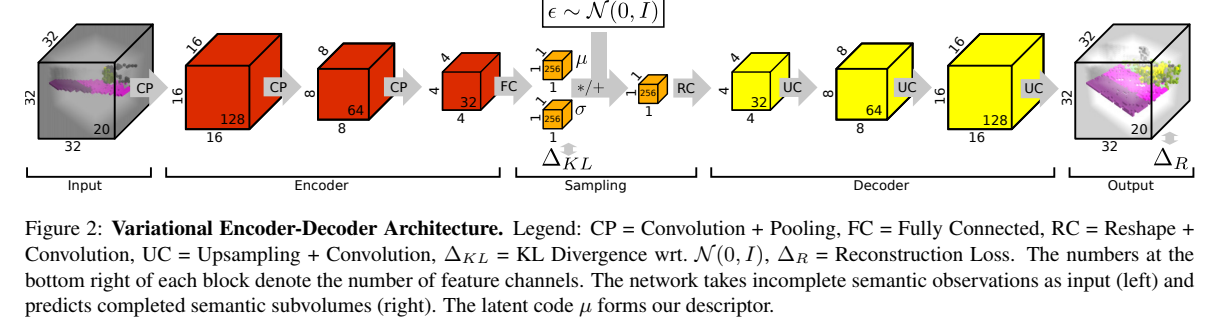
\includegraphics[width=0.85\textwidth]{SemanticSLAM/SemanticVisualLoc0.png}
\caption{Generative Descriptor Learning的示意图}
\label{SemanticVisualLoc0}
\end{figure}

\item Bags of Semantic Words

 Note that given an incomplete map, the bag of semantic words is a description of its complete
semantic scene layout. Our localization pipeline uses this representation to robustly match the query map to the database map, as detailed in the following.

这个bag of semantic words是通过计算属于$M$的所有subvolume来得到集合。也就是Encoder部分的输出构成的集合,具体得看论文吧。

\item Semantic Vocabulary for Indexing and Search

基于Euclidean metric来计算Query和Database之间的相似性,具体是利用Encoder部分的输出来计算距离。

\item Semantic Alignment and Verification

计算一组Query在不同Rotation下与Database之间的相似性,这些计算结果作为准确定位的基础,这就是这一小节要说明的内容。

通过类似于一种重投影误差的方式来判断计算的位姿的效果的好坏。

\end{itemize}

\subsection{Experiments}

用到了KITTI, NCLT数据集。

重复的场景结构容易引入Local Ambiguities, 会导致错误的定位。Global Ambiguities发生的较少,但会导致上百米的定位错误。通过考虑多帧的数据可以有效降低上述两种Ambiguities。此外,可以增加训练数据的多样性对于提高精度或许也有帮助。

\subsection{Conclusions}

In this paper, we proposed a novel method for localization using a joint semantic and geometric  understanding of the 3D world.

At its core lies a novel approach to learning robust 3D semantic descriptors. 

\section{小结3}

在前面两个小结的基础上,这里在强调一下几个重要的改进点!:

{\color{red} \bfseries 首先,实验目的是什么,有一些是实现Semantic SLAM, 也有提高定位信息的!然后,输入数据是什么, 现在趋势是借助多模态的数据,最经常用的是 Depth和RGB图像,此外,还有前面涉及到的Contour以及Semantic Information 和 3D Geometry信息,还有就是多帧数据实现非监督什么的。所以,一个可选的工作是,怎么把这些数据最高效的整合起来,可以借助RNN中的Gate思想,也可以看一下Knowledge 蒸馏法,以及Attention机制什么的!!!}

\section[StaticFusion]{StaticFusion: Background reconstruction for dense RGBD SLAM Dynamic Environments}

参考文献:\cite{scona2018staticfusion}

主要目的:提出一个鲁棒的、稠密的、基于RDBD的、可处理Dynamic Environment的 SLAM系统。

可以实现对Static和Dynamic Environment的分割,以及只对Static部分建模,来提高相机位姿估计的精度,降低overal drift的影响。

\subsection{背景}

现有的SLAM系统都假设场景是静态的,所以通过图像对之间的匹配可以得到相机的变换关系。但是现在场景中存在动态目标,那么图像之间的匹配就不单单是由于相机变换引起的了,所以需要区分静态场景和动态场景,并且动态场景对地图的构建也会产生不可逆的影响。

主要做了两件事:
\begin{itemize}
\item 同时估计相机的位姿以及对static和Dynamic场景的分割

其中,RGBD相机估计,通过把新来的图像帧与一个稠密的surfel-based SLAM model一起实现,如ElasticFusion。

\item 使用Static场景对环境进行了更具有一致性的建模
\end{itemize}

作者有公开源码。

\subsection{动态场景下SLAM系统的相关工作}

ElasticFusion是首个基于RGBD的SLAM系统,现在在Scalable estnesion、loop clusure capabilities、consider run-time limitations等方面改进,这一小节主要总结在Dynamic Environment场景下的一些改进方法。主要有三个方面:
\begin{itemize}
\item Implicit Handing of Dynamic Elements

这一类算法通过对High-residual points施加惩罚项来提高位姿估计的鲁棒性。其他的如ElasticFusion等算法在构建地图之前,需要目标在连续的多帧图像中都可以观察到,才会被认为是Static部分,加入到地图构建中。但这些算法并不会明确的对Dynamic Object进行处理,只能适用于运动物体在图像中范围比较小或者相机的运动幅度很小。

\item Outlier Rejection Strategies

一种常用的方法是把Dynamic moving object当做噪声来处理,被检测出来然后被滤波去除。

这一类的方法包括:DTAM、ORB-SLAM等。通过非常保守的关键帧选取策略来提高系统的鲁棒性。但这些算法并没有考虑在连续帧中检测Dynamic points是使用Spatial和temporal上面的Coherence。

{\color{red} \textbf{评语}:所以在Temporal上的Coherence可以使用RNN来帮助解决,而在Spatial上面的Coherence可以通过CRF之类的算法实现,最近不是也有ConvCRF的算法出现么!可以考虑考虑。}

\item Methods Enforcing Spatial on temporal Coherence

此外,还可以借助IMU以及Robot's odometry来提高Dynamic下的SLAM的鲁棒性,但本文主要基于单目RGBD相机来做。

\end{itemize}

\subsection{Framework和Notation}

主要的流程:
\begin{figure}[!hbtp]
\centering
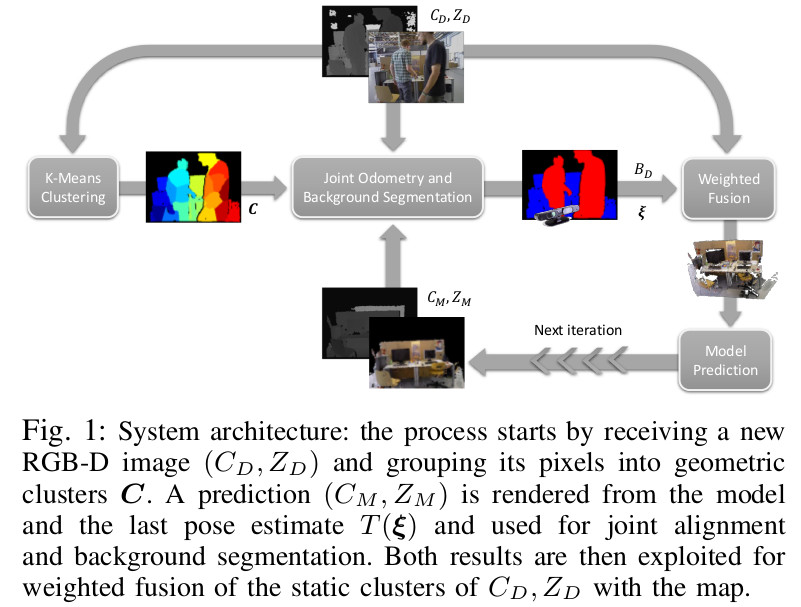
\includegraphics[width=0.75\textwidth]{SemanticSLAM/StaticFusion0.png}
\caption{StaticFusion算法的三个主要流程}
\label{StaticFusion0}
\end{figure}

三个步骤:
\begin{enumerate}
\item From incoming pair $I_D, Z_D$ 得到3D Geometry Cluters $\mathbf{C}$

其中, $C_D$是输入的彩色图像, $Z_D$是输入的Depth图像, $I_D$是基于$C_D$得到的Intensity image。这个分割算法来自于:Fast odometry and scene flow from RGB-D cameras based on geometric clustering.作者假设分割后的每一个cluster是rigid body.

\item 根据上一帧的相机位姿预测这一时刻的场景图片$C_M, D_M$, 然后这个预测结果与这一时刻实际的数据的分割结果来联合估计相机的运动$\xi \in \mathfrak{se}(3)$, 与此同时,这一步还会得到一个基于运动的场景分割,对于每一Cluster,我们分配一个Score, $b_i \in [0, 1]$, 来表示这一个Cluster属于Dynamic还是Static, 本文中,$b_i = 1$是Static, $b_i=0$是Dynamic, 在之间则表明不同程度的不确定性。

具体还会用到到上一时刻截止的Map信息。

\item 最后,利用上一步计算得到的$\xi$和运动分割结果, 得到一个pixel-wise的分割图\ref{StaticFusion0}中的$B_D$, 这一步只处理输入上一步计算的Static部分来计算。然后这个计算结果与输入$C_D, Z_D$进行加权\textbf{3D} Fusion。

\end{enumerate}

每一步的具体实现,还需要下面的讲解。

\subsubsection{第二步的计算}







\section{Convolutional CRFs for Semantic Segmentation}

参考文献:\cite{marvin2018crf}

之前的研究人员会用CRF作为语义分割的后处理步骤,但CRF有两个缺点:训练困难,推理计算速度慢。

为了解决这两个问题,作者在本文中提出在全连接CRF中引入条件独立性的假设。这样的后果就是,我们可以以卷积的形式重新组织CRF的推理计算过程,而且可以通过后向传播的方式在训练过程中优化模型参数。最终可以借助GPU进行加速训练,效果是速度可以提高两个数量级。

\subsection{背景 \& 相关工作}

传统用于语义分割的CNN的缺点是:只能提取局部特征,不能利用全局的Contexture。所以有人认为简单的前向CNN不能满足Structured Predictions类任务。

在FCN的基础上,Transposed convolution layer用于提高Feature Map的分辨率,Dilated convolutions用于提取空间信息(Spatial information)。很多网络结构都是基于这种思路来做的!而这一类做法严重依赖于CNN提取特征的能力,进行pixel-wise的预测。stuctured knowledge and background context被忽略。

一种在CNN中加入sturctured predictions into CNN的方法是在CNN的输出上加入fully-conneced CRF进行后续处理。Pyramid pooling是另一种与CRF类似作用的方法, 用于提高CNN的感受野,但并不会提供真正的structured reasoning。

还是那句话,主要是两个问题,那么现在有哪些方法来解决这两个问题呢?
\begin{itemize}
\item Parameter Learning in CRFs

一些方法包括:EM和Grid-search, Gradient Decent, Quadratic Optimization等。但都不太适合CNN的训练流程。

\item Inference speed of CRFs

一些方法输出降维的数据,但会影响预测能力。据作者所知,目前还没有一种可以有效提高FullCRFs推理速度的方法。

\end{itemize}

\subsection{Fully Connected CRFs}

CRF嘛,基于随机场的原理来实现的。首先说明下符号:$I$是输入图像,具有$\mathbf{n}$个像素;$\mathbf{X}\in \{ X_1, \ldots, X_n \}$表示每一个像素的标签,即分割结果中的类别;假设共有$k$个类别,即每一个$X_i$都有$k$个可能的取值。所以得到的条件随机场模型,以吉布斯分布的形式(基于成本函数表示的吧应该):
\begin{displaymath}
P(X=\hat{x}|\tilde{I}=I) = \frac{1}{Z(I)}\exp(-E(\hat{x}|I))
\end{displaymath}

其中,$E(\hat{x}|I)$表示能量函数,由下式给出:
\begin{displaymath}
E(\hat{x}|I) = \sum_{i \le N}\psi_u(\hat{x}_i|I) + \sum_{i\ne j \le N}\psi(\hat{x}_i, \hat{x}_j | I)
\end{displaymath}

上式中的第一项是Unary Potential,传统的来自于普通的CNN的语义分割结果可以认为就是这一项的具体取值了。那么还有后一项,后一项包含两个像素的分割结果,表示的就是利用Spatial Information了。重点说一下这一项。

后一项叫做Pairwise Potential,表示$\hat{x}_i, \hat{x}_j$的联合分布,这里的$x_i, x_j$其实也是可以是来自于CNN的语义分割预测结果,与Unary potential中的输入是一样的!可以用于明确表示这两个像素之间的联系,如近似的颜色等。在FullCRFs中,这一项是基于weighted sum of M个 gaussian kernels来实现的。
\begin{displaymath}
\psi(x_i, x_j | I) = \mu(x_i, x_j)\sum_{m=1}^{M}\omega^{(m)}k_G^{(m)}\left( f_i^I, f_j^I \right)
\end{displaymath}

其中,$\omega^{(m)}$是可以学习的参数,特征向量$f_i^I, f_j^I$可以任意选择,并可以依赖于输入图像$I$。但是最开始的那个函数$\mu(x_i, x_j)$是the compatibility transformation,只与$x_i, x_j$有关,而与输入无关。接下来重点说一下这个函数的选择。

一种普遍的选择是用Patts Model来做$\mu(x_i, x_j) = |x_i \ne x_j |$,关于这个模型,可以参考Wikipedia,我记得笔记中也有,但记不清了。而在CRFasRNN中,提出利用1*1的卷积来做Compatibility transformation。这样一种函数可以让模型学习更多的structured interactions between predictions。

说完了$\mu$函数,那么来看一下在FullCRF中,是怎么实现后面对Gaussian kernel的加权的吧。在FullCRF中,有两个Gaussian Kernelz作为hand-crafted features。Appearance kernel $k_\alpha$考虑了颜色的取值$I_i, I_j$作为特征; smoothness kernel基于spatial corrdinates$p_i, p_j$来实现。整个的Pairwise potential 由下式给出:
\begin{displaymath} 
k(f_i^I, f_j^I) = \omega^{(1)}\exp\left( -\frac{|p_i - p_j|^2}{2\theta_\alpha^2} -\frac{|I_i - I_j|^2}{2\theta_\beta^2} \right) + \omega^{(2)}\exp\left( -\frac{|p_i - p_j|^2}{2\theta_\gamma^2} \right)
\end{displaymath}

其中, $\omega, \theta$都是可以学习的参数。需要指出的是,这是一种Hand-crafted feature,有助于提高CRF的优化效率。

\subsubsection{Full CRF的Mean field inference}

FullCRF的推理主要基于Mean Field inference来实现的。具体步骤如图\ref{ConvCRF0}所示。

\begin{figure}[!hbtp]
\centering
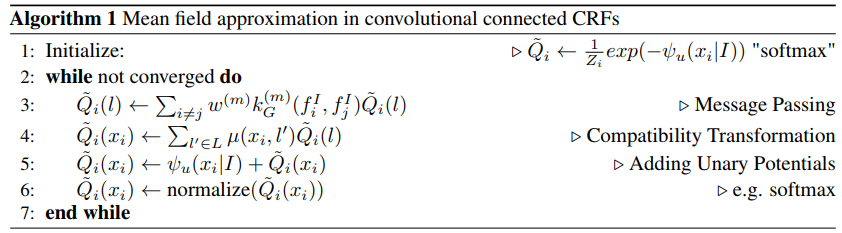
\includegraphics[width=0.85\textwidth]{SemanticSLAM/ConvCRF0.png}
\caption{Mean field inference算法步骤}
\label{ConvCRF0}
\end{figure}


对这个算法,简单说两句,除了message passing这一步之外,其它的几个步骤都是可以高度并行的。可以用GPU进行加速。 Message Passing也是CRF计算的瓶颈,计算量与输入图像的像素数的平方成正比,有研究人员提出利用Permutohedral lattice模型来近似,从而提高计算效率,这个近似模型是一种高维的滤波算法。但这种模型是基于一种很复杂的数据结构来实现的,存在基于CPU的复杂但快速的实现,但不适合GPU的实现。实际上,Permutohedral lattice模型的梯度求解也是一件很麻烦的事情,这也是为什么FullCRF之类的算法基于Hand-crafted features来做。

\subsection{Convolutional CRFs}

Convolution CRF其实就是在Full CRF的基础上引入了条件独立假设,即如果两个特征之间的Manhattan距离超过一个阈值$k$即$d(i, j) > k$那么就认为这两个点之间是独立的,这个$k$作者称为filter-size。

在Pairwise Potentional上面的体现就是,若大于这个阈值,$\psi_p$为0。

\subsubsection{Efficient Message Passing in ConvCRFs }

上面也提到了,Message Passing是CRF的计算瓶颈,本文提出的方法可以有效解决这个瓶颈,这是本文的主要贡献之一, 就不需要再使用Permutohedral模型近似了,也可以借助GPU加速计算了。为了实现这个目标,作者提出利用截断Gaussian Kernel实现的卷积操作来完成Message Passing这一步,这样就可以利用普通的CNN来完成了。

假设输入$P$是的尺寸是$[bs, c, h, w]$, 分别对应Batch size、通道数、高度、宽度。最终可以得到下面的公式,具体的构成看论文吧,那个公式有点复杂。

\begin{displaymath}
Q[b, c, x, y] = \sum_{dx, dy \le k} K[b, dx, dy, x, y] \cdot P[b, c, x+dx, y+dy]
\end{displaymath}

可以看出滤波器的取值还与Spatial dimension有关,需要注意的地方是,卷及操作实在通道为度上进行的。{\bfseries 这里进行的信号处理中的卷及操作,而不是NN中的卷及操作,后者其实是相关操作。}

这一步可以基于GPU来加速,但会涉及GPU中数据的重新组织,而实际上90\%的GPU运算时间都花在了数据重新组织上了。有一段关于卷积运算的阐述看论文。

\subsubsection{Additional implementation details}

ConvCRF中的设计策略与FullCRF中相同,即使用Softmax进行归一化、使用Potts model以及Hand-crafted gaussian featreu等。同样的,对Pairwise kernels做Gaussian blur,这样可以增加滤波器的有效大小变成4倍,这是为什么!

作者也实现了基于1*1卷积的实现,作为实验结果进行分析, 或者在Pairwise 中的输入换成可以学习的Feature数值。

使用VOC2012。使用ResNet101作为Unary potentials。

训练的时候,采用Decoupled Training的策略。即首先训练CNN模型,以语义分割为目标;然后固定CNN的输出,进行CRF的训练。

{\color{red} \bfseries 评语: 可以看得出来,作者是用CNN输出的完整分辨率的CRF进行训练的,这得多耗时,所以,下一步就是在Feature领域进行CRF操作!}


\subsection{总结}

通过增加条件独立的假设,我们可以去除Permutohedral lattice approximation,从而可以借助GPU完成高效的消息传递的计算,并是以卷积的方式进行。

下面,作者说还是要如何更好的捕获全局信息。也会把ConvCRF应用于Instance Segmentation以及Landmark recognition等应用中看一下效果怎么样!




\section[Co-Fusion]{Co-Fusion: Real time segmentation tracking and fusion of multiple objects}

参考文献:\cite{runz2017co}

输入的数据是RGBD, 主要通过对运动物体进行建模,完成场景的描述,可以作用在动态场景下。

表现在:把场景分割成多个Objects, 并实时的对他们进行跟踪和Shape建模。


\section{Squeeze-and-Excitation Networks}

参考文献:\cite{senet2017hu}

本文主要的关注点是如何更好的处理Channel-wise的信息。普通的卷及操作,会同时考虑局部的区域特征以及不同特征图之间的组合,而本文主要考虑Channel wise信息的提取,作者认为这样可以提高模型的表示能力!

具体结构如下图所示:
\begin{figure}[!hbtp]
\centering
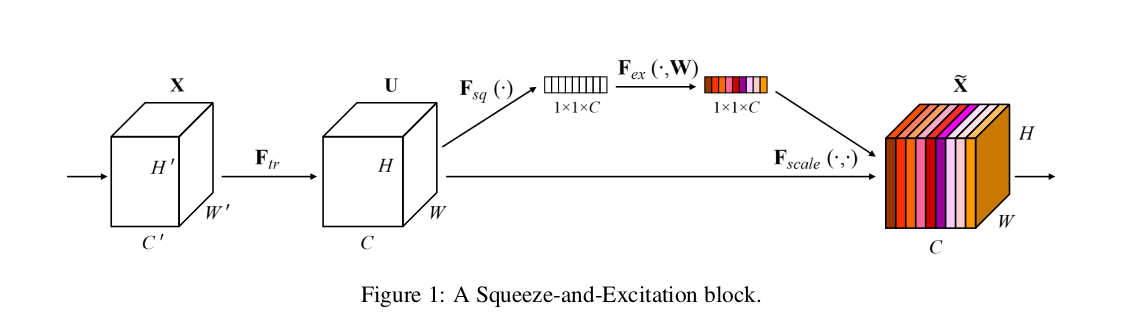
\includegraphics[width=0.85\textwidth]{SemanticSLAM/SENet0.png}
\caption{SENet结构示意图}
\label{SENet0}
\end{figure}

图\ref{SENet0}需要注意以下几点:
\begin{itemize}
\item $F_{sq}(\cdot)$表示文中所说的Sequeeze,这是基于Global Max Pooling (GAP)实现的,所以这一步并不会引入额外的参数,只又很少量的计算代价.这一步的结果就是输入的Feature Map编程$1 \times 1 \times C$的向量,作者把这个vector称为Channel Descriptor。
\item $F_{ex}(\cdot, \omega)$表示文中所说的Excitation,这是由Sigmoid和Bottleneck结构实现的。Bottleneck结构是两层具有不同输出维度的全连接层,可以表示成:
\begin{displaymath}
\mathbf{s} = F_{ex}(\mathbf{z}, \mathbf{W})=\sigma(g(\mathbf{z}, \mathbf{W})) = \sigma(\mathbf{W}_2 \sigma (\mathbf{W}_1 \mathbf{z}))
\end{displaymath}


其中$\sigma$为ReLU,$W_1 \in R^{\frac{C}{r}\times C}$, $W_2 \in R^{C \times \frac{C}{r}}$, 其中C表示输入Feature Map的通道数,也就是$\mathbf{U}$的通道数,这一结构也称为Bottleneck,是为了降低参数数量,r是ratio,作者实验证明了可以选择16。

\item $F_{scale}(\cdot, \cdot)$表示Channel-wise的相乘

\item 作者的实验表明,这个S-and-E Block放在网络结构的中部、前部比较好,放在后面效果不是特别很好,但会增加比较多的参数,因为后面的通道数C比较大,所以可以去掉。这是基于ResNet验证的。
\end{itemize}

如何把SE Block加入到ResNet等网络中,可以看文章。

\section{Deep Multi-scale Architectures For Monocular Depth Estimation}

参考文献:

本文主要回顾使用Multi-scale的网络结构进行深度估计,表明相比于只使用一种Scale的Feature,可以提高精度、定性上更好的深度图。在NYU Depth上实现了SOTA。

\subsection{背景与相关工作}

有学者指出,受人类视觉的激发,发展了一些算法,人类视觉会利用Texture, Perspective, defocus等信息。

最早的两篇基于深度学习来做的工作是:

\begin{itemize}
\item Deep Deconvolutional Networks for Scene Parsing
\item Depth map prediction from a single image using a multi-scale deep network
\end{itemize}

基于这两个工作,后面提出了非常多的改进方法,但比较少关注多尺度问题。本文的实验表明,如果在小的数据集上,多尺度网络可以比精心设计的单尺度网络更好一点的话,那么在打的数据集上,就会有SOTA结果。

相关工作有:
\begin{itemize}
\item Depth map prediction from a single image using a multi-scale deep network, 2014

网络结构包含两个部分,由两个网络Stack而成。第一个网络输出Coarse depth map, 第二个网络对输出的这个粗糙的深度图进行Refines, 后一个网络通过3 successive卷积实现,用Coarse depth map和RGB image作为输入。

\item Predicting depth, surface normals and semantic labels with a common multi-scale convolutional architecture. 2015

增加了一个新的CNN模块,同时多任务预测。

\item Towards unified depth and semantic prediction from a single image, 2015

使用语义信息帮助深度估计。

\item Learning depth from single monocular image using deep convolutional neural fields, 2016

\item Deep convolution neural fields for depth estimation from a single image, 2015

\item Depth and surface normal estimation from monocular images using regression on deep features and hierarchical crfs. 2015

\item Monocular depth estimation using neural regression forest. 2015

\item Depth from a single image by harmonizing overcomplete local network predictions, 2016

\item Deeper depth prediction with fully convolutional residual network, 2016

Encoder-decoder network。 实验表明使用BerHu loss可以提高精度。是下了SOTA的实验结果。

\end{itemize}


\section{Depth Map Prediction from a single image usign a multi-Scale Deep Network}

参考文献:

基于单目图像预测深度需要来自于多个Cues的both global and local信息。本文的两个主要贡献:
\begin{itemize}
\item 提出利用two network stack完成深度预测,一个完成coarse global prediction based on entire image, 另一个完成refines this prediction locally.
\item 提出一个scale-invariant error,帮助测量深度
\end{itemize}

整体结构如图\ref{DepthPrediction2014_0}所示:
\begin{figure}[!hbtp]
\centering
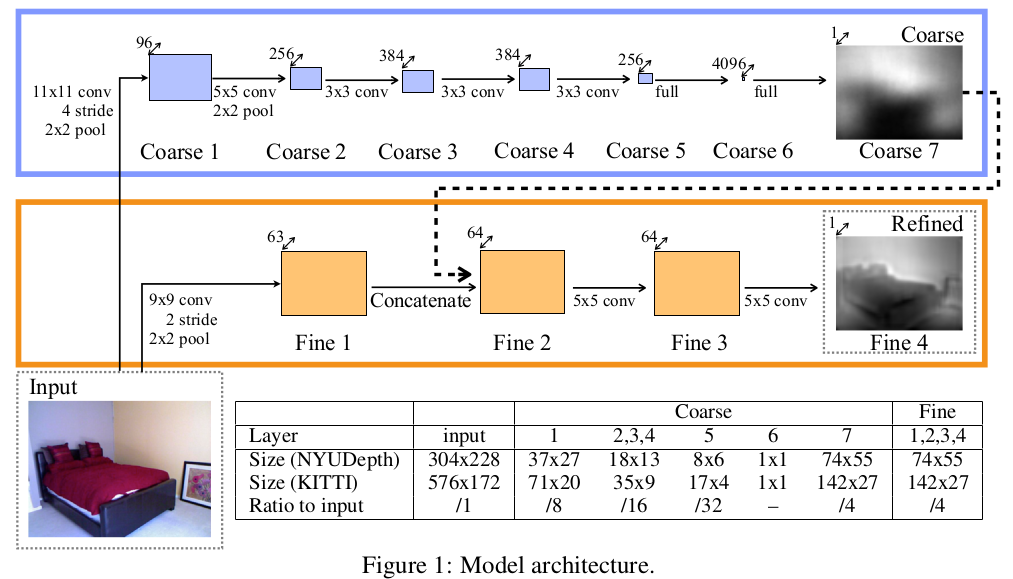
\includegraphics[width=0.85\textwidth]{SemanticSLAM/DepthPrediction2014_0.png}
\caption{网络结构示意图}
\label{DepthPrediction2014_0}
\end{figure}

在第一个部分,也就是得到Coarse Depth Map的部分,通过全连接层实现输入图像的全局视野,此外,在中间几层使用Max Pooling增加局部的感受野。但有一地方是如何根据Coarse6的输出得到Coarse7。作者也没说明白!全连接中还应用了Dropout。

在第二部分,首先对输入图像进行一次卷积运算,然后结果与上面的Coarse7的输出进行Concatenate,后面的卷积运算都会有Zero padding保持输出的大小一致。

第二个贡献是提出了一个Scale-Invariant Error (Metric), 因为单目预测深度的时候会有尺度问题,所以作者用下面的公式:
\begin{displaymath}
D(y, y^{*})  = \frac{1}{2n}\sum_{i=1}^{n} \left( \log y_i - \log y^{*}_i  \alpha(y, y^{*}) \right)^2
\end{displaymath}
其中,$ \alpha(y, y^{*})= \frac{i}{n}\sum_{i}(\log y_i - \log y^{*}_i)$.$n$为像素的个数,$i$为像素的索引。

最后作者的目标函数就是基于这个Scale-Invriant Error来做的。

\begin{displaymath}
See the paper.
\end{displaymath}

由于网络最后的输出是下采样了4倍,所以,在训练的时候需要把depth和mask都直接下采样比例为4。

\section{Mask R-CNN}

参考文献:\cite{maskrcnn2017he}

这篇文章的重要贡献是实现了Instance-Level的语义分割,具体是实现实在Faster-RCNN的基础上,新增了一个Branch用于预测Object Mask。它与物体检测(Object Detection)的区别是,提供Mask的预测结果而不是Boundingbox;它与语义分割的区别是,它是Instace-level的分割,而不是像素级的、不区分Instance的分割。

示意图如图所示:
\begin{figure}[!hbtp]
\centering
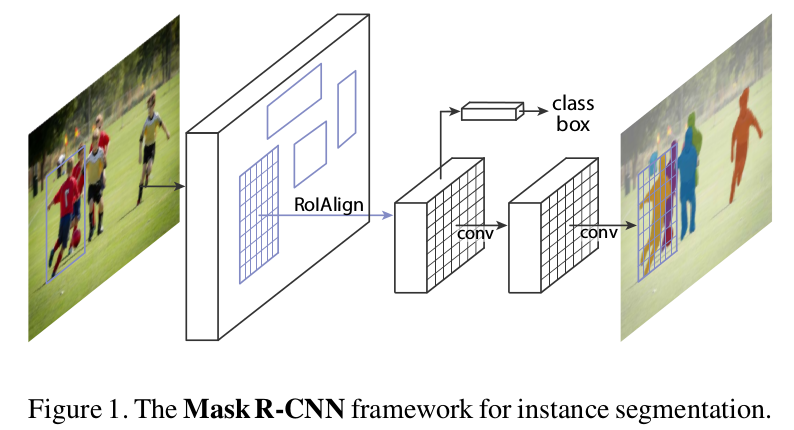
\includegraphics[width=0.85\textwidth]{SemanticSLAM/MaskRCNN0.png}
\caption{Mask RCNN示意图,在class box的基础上增加了预测mask的分支。}
\label{MaskRCNN0}
\end{figure}

\subsection{研究现状与相关背景}

在Faster-RCNN的基础上实现的,但是由于Faster-RCNN中的RoI Pooling会导致网络的输出与输入并不是Pixel-by-pixel的Alignment, 所以,在得到Mask的时候,作者提出利用RoIAlign的结构,可以faithfully preserves exact spatial locations.

{\bfseries 非常重要的一点是:mask和class 的预测是分离的(decouple)的两个过程,而FCN之类的算法是既需要perform per-pixel multi-class categorization, which couples segmentation and classification,后一种方式对Instance segmentation的效果较差。}


\subsection{Mask RCNN}

主要有以下几点需要注意的地方:
\begin{itemize}
\item 使用ROIAlign层代替原来的ROI Pooling层
\item 分离Region Proposal的分类+BBox回归 和 像素级的语义分割
\item 第三条Branch输出的二值的图像,然后与Class Prediction的结果一起计算误差
\end{itemize}

主要想明白这一点:就是如何对齐的问题!

为什么在SPP Net和Fast RCNN中的ROI Pooling会对不齐呢,有两个方面的原因:
\begin{itemize}
\item 因方面由于存在Pooling的降维计算,会求除法一次
\item 在Spatial Pyramid Pooling产生固定大小的输入的时候(在Mask RCNN论文里面叫做bin),还会求除法一次
\end{itemize}

那么具体是怎么操作的呢:

参看文献:\href{https://zhuanlan.zhihu.com/p/26652657}{CNN图像分割简史-知乎}

\begin{figure}[!hbtp]
\centering
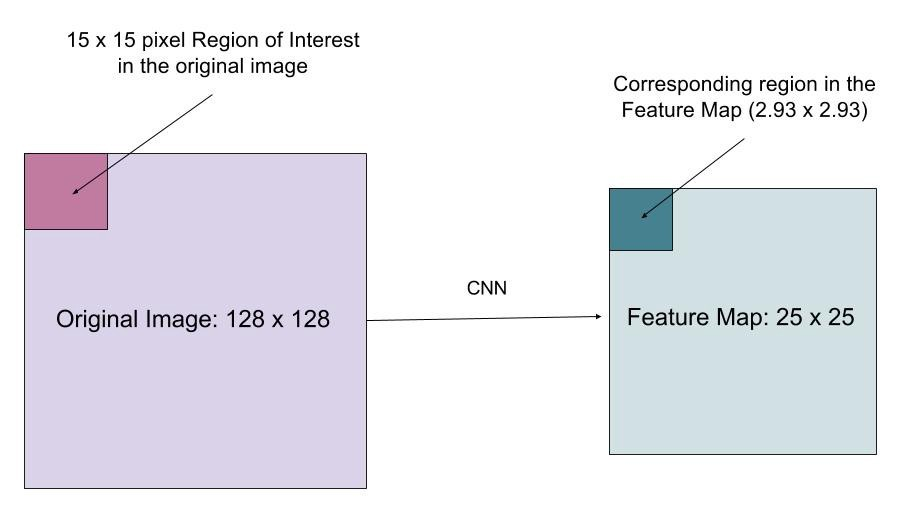
\includegraphics[width=0.75\textwidth]{SemanticSLAM/MaskRCNN1_ROIAlign0.jpg}
\caption{ROI Align的示意图, 如何将region of interest的原始图像和特征图精确对齐?}
\label{MaskRCNN1_ROIAlign0}
\end{figure}

假设有一幅128*128大小的图像,对应的特征图大小为25*25,如果要将原始图像左上角15*15大小的像素映射到特征图中(如图16所示),如何从特征图中选择像素呢?显然原始图像中每个像素对应特征图中的25/128个像素,要选择原始图像中的15个像素,需要选择15*25/128=2.93个像素。

在RoIPool中,我们会四舍五入选择3个像素,从而会导致微小的偏移。在RoIAlign中,我们要避免这样的近似。取而代之的是采用bilinear interpolation获取精确的对应值,即选择像素2.93,从而能够避免RoIPool导致的偏移。

\subsection{实验}

使用Averaged over IoU thresholds来计算。AP是Average Precision的意思,只不过这里只有当IoU与Ground Truth重叠到一定程度后才认为是分类正确的,作者用到的:$AP_{50}, AP_{75}$等。

\subsection{总结}

基于Faster RCNN实现的Mask RCNN可以出人意料简单的解决Instance Segmentation问题。

\section{Learning to segment every thing}

参考文献:\cite{hu2017learning}

本文非常值得再读。

需要注意的几个亮点:
\begin{itemize}
\item 提出了基于Transfer Learning的Partially supervised instance segmentation功能,可以实现3000个种类的Instance的分割。
\item 与以往不同的是,作者是在Mask RCNN中Detection Branch Head部分的权重的基础上进行迁移学习的,学习Segmentation Head的权重参数!以往的做法可以是利用Word2Vec 或 GloVe等算法把Feature Map映射到Embedding空间中进行迁移学习,这也是Zero Shot Learning中的做法。
\item 那么具体是怎么实现从Detection Head的圈中参数迁移到Segmentation Head部分的权重参数的呢。作者比较了两种思路:利用一个仿射变换实现、利用两三层的神经网络(MLP)+LeakyReLU来做。Ablation测试发现后者更好
\item 前面说到了,作者测试了集中迁移结构的输入,包括Detection Head的Feature 输出、NLP算法输出的Embedding、DetectionHead的权重参数,Ablation实验发现后者更好。
\item 需要值得注意的是,作者认为MLP的Head更适合Category Agnostic,FCN更适合Class-specific的分割,所以他们两个算法可以互补!
\item 训练数据分成了两组,一组具有精确地Segmentation Mask,一组只有Bounding box。
\item 比较了两种不同的训练策略。Stage Wise, 即先训练Faster RCNN部分,然后固定参数再训练Segementation任务;End-to-End训练,即整个模型一起训练,但是在训练Segmentation Head的样本时,不能对Detection Head部分的权重进行更新!
\item 存在扩展到Open Set Recogntion的论文:Bayesian Semantic Instance Segmentation in Open set World.
\end{itemize}

暂时就只有以上几点。

论文思路的整体框架如图所示:
\begin{figure}[!hbtp]
\centering
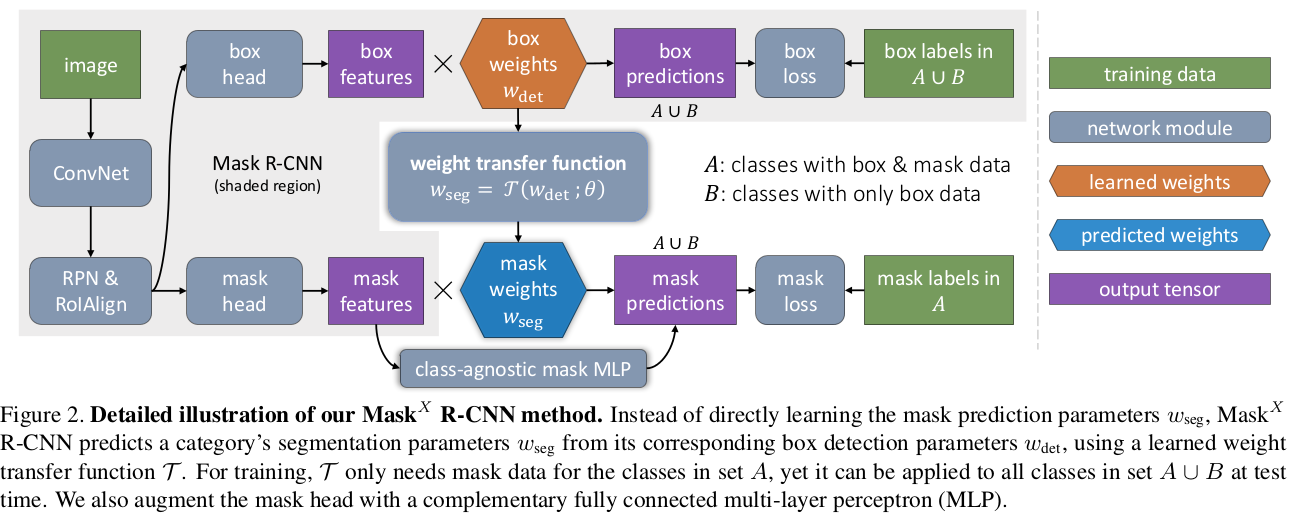
\includegraphics[width=0.95\textwidth]{SemanticSLAM/MaskXRCNN0.png}
\caption{论文的整体结构,包括Weight Transfer 结构}
\label{MaskXRCNN0}
\end{figure}

其中Weight Transfer结构的数学表达式是:
\begin{displaymath}
\omega_{seg}^c = \mathcal{T}(\omega_{det}^c; \theta)
\end{displaymath}

其中,$\omega$是权重,$\omega_{det}$来自于Mask RCNN中的Detection Head, 论文作者通过把用于分类的权重$\omega_{cls}$和用于BBox回归的权重$\omega_{box}$进行Concatenate构成$\omega_{dec}$。

\section{Path aggregation network for instance segmentation}

参考文献:\cite{liu2018path}

根据论文题目也可以看出,作者主要的改进的是Path Aggregation. 也就是增加了Bottom->top的Feature Pyramid, 实在FPN的基础上实现的,也就是说本身就包含一条Top->Bottom的Path。

此外,作者针对Mask RCNN中的三个问题,提出了三个改进的办法!


有时间把论文细节补上。还是有很多值得学习的地方的。

{\color{red} \bfseries 自从ResNet火起来后,这个Path Aggregation的方式貌似用的挺多的,关键还是让不同Level的feature更方便的信息交流!比如在本文中,低层次的Feature也可以支持Large Object, 高层次的Feature也可以支持Small Object。}


\section{End-to-End Instance Segmentation with Recurrent Attention}

参考文献:\cite{ren2017end}

比较有意思的几点:

在图像预处理过程中,作者用FCN输出两类数据,一类是1个Channel的前景分割;另一类是每一个Object的Angle Map, 作者把这个角度分成八个方向。为什么也会输出Angle Map呢?因为作者认为:Predicting the angle map forces the model to encode more detailed information about object boundaries。

{\color{red} 所以通过多任务学习、改进Loss函数,可以有效提高多任务中的单个任务的性能。我猜测,这个多任务肯定得是具有某种同性的作用,通过多个任务之间的共同的约束来提高单一任务的性能,或者强迫模型学习得到我们想要的性质!}

现在这个智商啊,下降的非常厉害。

\section{Fully Convolutional Instance-aware Semantic Segmentation}

参考文献:\cite{li2016fully}

同时检测、分割Instances。引入了Positioin-senstive inside/outside score maps, 两个任务的底层卷积表示是完全Shared的。

\subsection{背景与相关现状}

Extends the translation invariant score maps in conventional FCNs to \textit{position-sensitive} score maps, which are somewhat translation-variant.

也就是说抛弃了以往的Translation invariant, 而是加上了部分的Translation Variant性质(在分割的时候这样做)。

\subsection{Our Approach}

为了在Mask Prediction中引入Translation-variant性质,作者用了一个Fully Convolution solution来实现Instance Mask Proposal。

作者总结到,高性能的原因来自于高度集中和高效的网络结构,尤其是联合训练Classification和Mask Segmentation的思想。

那么是怎么整合到一起的呢?作者说是通过Fuses the two answers into two scores. 此外,提高Position-sensitive score map的想法来联合的和同时地完成Object segmentation和Detection两个任务。

所以,在深度学习中,重要的点还包括:网络结构 + 适合自己任务的Loss Function。对于后者,应该想明白怎样才是适合自己的Loss Function.

\section{TernausNetV2: Fully Convolutional Network for Instance Segmentation}

参考文献:\cite{iglovikov2018ternausnetv2}

作者利用Encoder-Decoder结构实现了对遥感数据的Instance-level Semantic Segmentation。 输入除了普通的RGB数据,还包括其它通道的数据。

\subsection{背景及相关工作}

首先提出了FCN结构用于语义分割,后来通过引入Skip Connections来允许综合low-level的Feature maps 和 higher-levle ones,可以保证精确地Pixel-level localization。 后者的典型是U-Net。

作者的方案是,在RGB上进行迁移学习,输出Semantic Mask后在用额外的Output Channel用于Predict areas where objects are touched or close to each other. 最后输出的是Separate Instances.

用到的数据集是SpaceNet。

\subsection{Model}

采用Encoder-Decoder的U-Net网络结构,并且作者把Encoder部分替换成 WideResNet-38 Network,后面这个结构具有In-place activated batch normalization的特点。In-palce activated Batch Normalization把Batch Normalization layer和Activation Layer合并到一起了,可以节省50\%的GPU存储空间。

此外,相比于ResNet, WideResnet每次卷积具有更多的输出Channel, 同时具有更浅的卷积层数。

而在Decoder部分,采用Nearest Neighbor Upsampling来实现分辨率的翻倍。

\subsection{Training}

再输入中,比3个通道多出来的几个通道的网络权重被初始化为0。

在第一个Epoch, 固定Encoder部分的权重,然后只训练Decoder部分的权重。在第二个Epoch开始, 训练所有的权重。作者认为,这样网络可以轻松的从3个通道学习扩展到多个通道的学习, 并且学习的过程是:Delicate, careful manner, slowly increasing weights of the multi-spectral part of the input.

作为Loss function, 作者采用了下面的损失函数:
\begin{displaymath}
L = \alpha H - (1 - \alpha)(1 - J)
\end{displaymath}

其中J是Jaccard loss, H是普通的交叉熵损失函数。

这个Jaccard loss具体长下面这样:
\begin{displaymath}
J = \frac{1}{n}\sum_{c=1}^{C}\omega_c \sum_{i = 1}^{n}\left( \frac{y_i^c \hat{y}_i^c}{y_i^c + \hat{y}_i^c - y_i^c \hat{y}_i^c} \right)
\end{displaymath}

其中, $\hat{y}$是预测的Mask, $y$是真实的Mask, $n$是每一个通道的像素数, $C$是总的通道数, 也就是类别数。






\subsection{常用数据集}

\subsection{KITTI}

数据集官网:\href{http://www.cvlibs.net/datasets/kitti/index.php}{KITTI Dataset}

参考文章:

[1] \href{https://blog.csdn.net/Solomon1558/article/details/70173223}{KITTI数据集简介和使用-CSDN}

KITTI数据集由德国卡尔斯鲁厄理工学院和丰田美国技术研究院联合创办,是目前国际上最大的自动驾驶场景下的计算机视觉算法评测数据集。该数据集用于评测立体图像(stereo),光流(optical flow),视觉测距(visual odometry),3D物体检测(object detection)和3D跟踪(tracking)等计算机视觉技术在车载环境下的性能。KITTI包含市区、乡村和高速公路等场景采集的真实图像数据,每张图像中最多达15辆车和30个行人,还有各种程度的遮挡与截断。整个数据集由389对立体图像和光流图,39.2 km视觉测距序列以及超过200k 3D标注物体的图像组成[1] ,以10Hz的频率采样及同步。总体上看,原始数据集被分类为’Road’, ’City’, ’Residential’, ’Campus’ 和 ’Person’。对于3D物体检测,label细分为car, van, truck, pedestrian, pedestrian(sitting), cyclist, tram以及misc组成。

\subsection{官网资源介绍}

最官网页面顶部,一共分了13栏,如图\ref{KITTI0}所示。

\begin{figure}[!hbtp]
\centering

\includegraphics[width=0.75\textwidth]{SemanticSLAM/KITTI0.png}
\caption{KITTI官网截图}
\label{KITTI0}
\end{figure}

其中,这些栏分别对应不同的应用目的提供单独的数据集,如Stereo, flow, sceneflow, depth, odometry, object, tracking, road, semantics, row data等。其中前三个貌似是对应同一个数据集。在depth中会有深度预测和深度补全等功能,semantics等包含一些标注好的图像数据等。Odometry等数据集比较大!

此外,作者还提供了一个Submit results栏,可以上传自己的测试结果等。但不能造假,即训练过程中,需要自己负责把训练数据分成train data 和 validate data, 然后用test data对模型进行测试。

\subsection{详述}

主要参考本小节的参考文章。

原始数据采集于2011年的5天,共有180GB数据。 

\subsubsection{组织形式}

图所示为早期的数据组织形式,与目前KITTI数据集官网公布的形式不同。在这早期的版本中,一个视频序列的所有的传感器数据都存储于data\_drive文件下, 其中data和driver是占位符,表示采集数据的日期和视频编号。时间戳记录在Timestamps.txt文件中。

\begin{figure}[!hbtp]
\centering
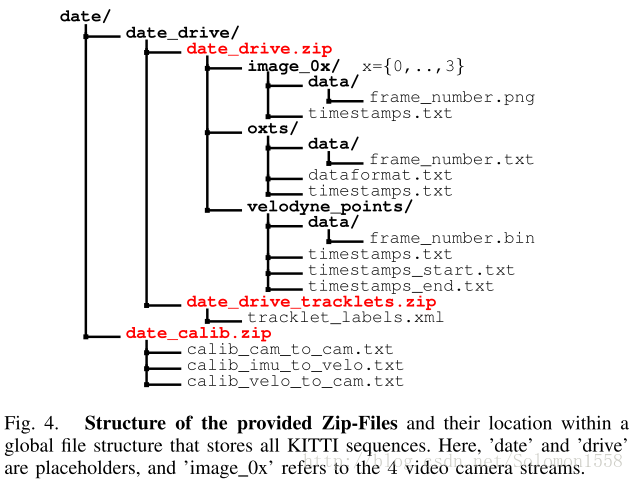
\includegraphics[width=0.75\textwidth]{SemanticSLAM/KITTI1.png}
\caption{早期的数据文件组织格式}
\label{KITTI1}
\end{figure}

而现在,对于从官网下载的各个分任务的数据集,其文件组织形式比较简单,以Object Detection为例,下面是Object detection Evaluation 2012 标准数据集中left color images 文件的目录结构,样本分别存储在testing和training数据集中。

\begin{verbatim}
data_object_image_2/
| -- testing/
|      | -- image_2/
| -- training/
|      | -- image_2/
|      | -- label_2/
\end{verbatim}

\subsubsection{Development Kit}

KITTI各个子数据集都提供开发工具 development kit,主要由cpp文件夹,matlab文件夹,mapping文件夹和readme.txt组成。

cpp文件夹主要包含评估模型的源代码evaluate\_object.cpp。Mapping文件夹中的文件记录训练集到原始数据集的映射,从而开发者能够同时使用激光雷达点云,gps数据,右边彩色摄像机数据以及灰度摄像机图像等多模态数据。Matlab文件夹中的工具包含读写标签,绘制2D/3D标注框,运行demo等工具。Readme.txt文件非常重要,详述介绍了某个子数据集的数据格式,benchmark介绍,结果评估方法等详细内容。

\subsection{Cityscape}

数据集官网:\href{https://www.cityscapes-dataset.com/}{Cityscapes Datasets}



\subsection{TUM}

数据集官网:\href{https://vision.in.tum.de/data/datasets}{TUM Datasets}

\section{实例分割-图像分割2018.06.11博客总结}

\subsection{Mask R-CNN狙击目标实例分割}

参考文献:\href{https://zhuanlan.zhihu.com/p/26047813}{Mask R-CNN 狙击目标实例分割-知乎}

\subsubsection{什么是实例分割}

举例子的方式:简单讲,一群人在图片里面,我希望把\textbf{每个人}都给我分割出来。分类只能做到识别这个图片是人;目标检测只能检测到这个图片里有人,把人的地方框出来,对每一个人这个个体不一样是没有判断的,统一认为是人;而图像分割主要是将人和背景分割出来,而实例分割就是要把每个人清晰的分割出来。

总的来说,Mask R-CNN是基于Faster R-CNN的基于上演进改良而来,FasterR-CNN并不是为了输入输出之间进行像素对齐的目标而设计的,为了弥补这个不足,我们提出了一个简洁非量化的层,名叫RoIAlign,RoIAlign可以保留大致的空间位置,除了这个改进之外,RoIAlign还有一个重大的影响:那就是它能够相对提高10\%到50\%的掩码精确度(Mask Accuracy),这种改进可以在更严格的定位度量指标下得到更好的度量结果。第二,我们发现分割掩码和类别预测很重要:为此,我们为每个类别分别预测了一个\textbf{二元}掩码。

\subsubsection{Mask RCNN介绍}
Mask R-CNN拥有简洁明了的思想:对于Faster R-CNN来说,对于每个目标对象,它有两个输出,一个是类标签(classlabel),一个是边界框的Offset(bounding-box offset),在此基础上,Mask R-CNN方法增加了第三个分支的输出:目标掩码。目标掩码与已有的class和box输出的不同在于它需要对目标的空间布局有一个更精细的提取。

\subsubsection{Mask RCNN的工作机理}

在Faster RCNN中,相比于Fast RCNN,多了一个Stage,那就是Region Proposal Network。所以在Faster RCNN中,整个算法由两个Stage构成,第一个Stage, 就是RPN, 这一步产生ROI,前面也提到了,在Fast RCNN中,输入既包括Image也包括一个ROI, 所以这里采用RPN来生成ROI。在第二Stage中,其实和Fast RCNN是一样的,都是借助ROI Pool来完成目标检测(目标分类+Bounding box offsets)。

那么在Mask RCNN中,在第二步骤中,与预测目标类别与Offset\textbf{平行的是}还会对每一个ROI输出一个Binary mask。所以Mask的branch, 会输出一个K*m*m大小的张量,其中K表示类别的个数。在实现过程中,

相应的,在训练的时候,也会采用一个多任务Loss Function:
\begin{displaymath}
L = L_{cls} + L_{box} + L_{mask}
\end{displaymath}

前两个Loss和Fast RCNN中是一样的,后面的mask的loss。有很多不懂的地方啊。

\subsubsection{Tensorflow + Keras实现实例分割}

参考文献:\href{https://mp.weixin.qq.com/s/Fo1yd6W1EdCQGEflP26tHA}{Tensorflow+Keras实现实例分割-微信公众号}

分割掩码是输入目标的空间布局编码,不像类别标签或边界框偏移量那样将特征经过全连接层“坍缩”到短的输出向量,而是自然地采用卷积实现“像素到像素”的变换,抽取掩码空间结构信息。使用 FCN 网络为每个 RoI 预测一个 mxm 掩码,这样允许它们保持 mxm 目标空间布局信息。

Mask RCNN 中使用 RoIAlign 替换了 RoIPool,RoIPool 没有考虑保留尽可能多的空间布局信息,难以实现输入图片/输出掩码像素一一对应。


\section{无需Proposal的实例分割论文}

参考文献:\href{https://zhuanlan.zhihu.com/p/35770716}{一文介绍3篇无需Proposal的实例分割论文-知乎}

基于Proposal(如:Mask R-CNN, MaskLab, PANet)的实例分割有三个根本缺陷:
\begin{itemize}
\item 两个物体可能共享同一个或者非常相似的边界框,此时,Mask Head无法区分要从边界框中拾取的对象。这对于其所在的边界框中具有地填充率的线状物体(如自行车和椅子)而言是非常严重的问题。
\item 架构中没有任何能够阻止两个共享像素的东西的存在
\item 实例的数量通常首先与网络能够处理的Proposal数量
\end{itemize}

前两点是什么意思?

文章列出了三篇通过距离学习的Instance Segemantation,貌似文章的作者称之为实例嵌入。
\begin{itemize}
\item 基于判断损失函数的语义实例分割,使用了非成对的损失函数。使用图像中所有像素产生了特别丰富的梯度。

 Semantic Instance Segmentation with a Discriminative Loss Function

\item 基于深度度量学习的实例语义分割,引入了种子模型,同时帮助我们分类并拾取最佳种子,做了速度优化。

Semantic Instance Segmentation via Deep Metric Learning

\item 用于实例分组的递归像素嵌入,GBMS是均值漂移的一种变体,在网络内部用于训练和解析。创建了非常密集的聚类。

(用于实例分组的递归像素嵌入)

\end{itemize}

他们比Proposal方法更简单,也可能更快,同时避免了Proposal的实例分割架构存在的三个根本缺陷。但实际效果并不如Proposald的方法。

此外,作者还给出了一些其它的方法的论文:
\begin{itemize}
\item 基于循环注意力机制的端到端实例分割(End-to-End Instance Segmentation with Recurrent Attention)
\item 用于实例分割的深分水岭变换(Deep Watershed Transform for Instance Segmentation)
\item 联合嵌入:用于联合检测和分组的端到端学习(Associative Embedding: End-to-End Learning for Joint Detection and Grouping)
\item 用于实例分割的序列分组网络(SGN: Sequential Grouping Networks for Instance Segmentation)
\end{itemize}



















